\documentclass[11pt,preprint]{report}

%\includeonly{introduction} 
\counterwithout{footnote}{chapter}

\usepackage{hyperref}
\hypersetup{
    colorlinks=true,
    linkcolor=black,
    filecolor=magenta,      
    urlcolor=blue,
    citecolor=black,
    %pdftitle={},
    pdfpagemode=FullScreen,
    }

\urlstyle{same}

\usepackage{array}

\usepackage{geometry}
 \geometry{
 a4paper,
 total={170mm,257mm},
 left=20mm,
 top=20mm,
 }
 
 \usepackage{graphicx}
 \graphicspath{ {figures/} }
 
\usepackage{amsmath, amsfonts}

\usepackage[toc,page]{appendix}

\usepackage{subfig}
 
 \usepackage[
 natbib=true, 
backend=biber,
style=authoryear,
sorting=nty,
maxcitenames=1
]{biblatex}
\addbibresource{bibliography.bib}
\renewcommand*{\nameyeardelim}{\addcomma\space}
\bibstyle{plain}

\renewenvironment{abstract}
 {\cleardoublepage\thispagestyle{empty}\null\vfill
  \begin{center}
  \bfseries \abstractname\vspace{-.5em}\vspace{0pt}
  \end{center}
  \list{}{
    \setlength{\leftmargin}{3cm}%
    \setlength{\rightmargin}{\leftmargin}%
  }%
  \item\relax}
 {\vfill\null}
 {\endlist}
 
\newenvironment{acknowledgements}
 {\cleardoublepage\thispagestyle{empty}\null\vfill
  \begin{center}
  \bfseries Acknowledgements\vspace{-.5em}\vspace{0pt}
  \end{center}
  \list{}{
    \setlength{\leftmargin}{2.5cm}%
    \setlength{\rightmargin}{\leftmargin}%
  }%
  \item\relax}
{\vfill\null}
{\endlist}

\begin{document}
\begin{titlepage}
\begin{center}
\hspace{0cm}
%\vspace{5cm}
\vspace{3cm}

\Large
Master's thesis in Data Science
\vspace{0.25cm}

\rule{\textwidth}{1pt}
\LARGE
%Semantic and object instance segmentation, and classification of tables in large-scale newspaper archives
\textbf{Automatic table detection and classification in large-scale newspaper archives}
\vspace{0.5cm}
\rule{\textwidth}{1pt}
   
\vspace{0.5cm}

\Large
Ecole Polytechnique Fédérale de Lausanne \\
\vspace{0.2cm}
\large
School of Computer and Communication Sciences\\
\vspace{0.2cm}
\large
Digital Humanities Laboratory \\


\vfill

\LARGE
\textbf{Arthur Vernet} \\
\vspace{0.25cm}
\large
Lausanne, 14th of January 2022
      
\vspace{2.5cm}

\includegraphics[width = 0.125\textwidth]{epfl.png}

\vspace{1.5cm}

\large
Supervisors: Maud Ehrmann (EPFL) and Simon Clematide (UZH).\\
\vspace{0.2cm}
Professor: Frédéric Kaplan (EPFL).
\vspace{1cm}
\end{center}
\end{titlepage}


\begin{abstract}
In recent decades, major efforts to digitize historical documents led to the creation of large machine readable corpora, including newspapers, which are waiting to be processed and analyzed. Newspapers are a valuable historical source, notably because of the plurality of subjects and points of view they cover; however their heterogeneity due to their diachronic properties and their visual richness makes them difficult to deal with. Certain recurring elements, such as tables, which are powerful layout objects because of their ability to easily convey a large amount of information through their logical visual arrangement, play a role in the difficulty of processing them. \\
This thesis focuses on automatic table processing in large-scale newspaper archives. Starting from a large corpus of Luxembourgish newspapers annotated with tables, we propose a statistical exploration of this dataset as well as strategies to address its annotation inconsistencies and to automatically bootstrap a training dataset for table classification. We also explore the ability of deep learning methods to detect and semantically classify tables. The performance of image segmentation models are compared in a series of experiments around their ability to learn under challenging conditions, while classifiers based on different combinations of data modalities are evaluated on the task of table classification. \\
Results show that visual models are able to detect tables by learning on an inconsistent ground truth, and that adding further modalities increases classification performance. 
\end{abstract}

\begin{acknowledgements}
An immense thank you goes out to my two supervisors for their invaluable guidance throughout this project, but also for their infectious dedication to the project. They helped me a great deal in understanding how to structure my thoughts and processes to best meet the scientific and academic standard.\\
A classic yet unavoidable thank you must go to both of my parents for their continued support and absolute confidence in my ability to complete my studies, even when their trajectory could not exactly be described as direct.\\
I would also like to thank the members of the DHLAB for their great hospitality and energy, which made me feel welcomed from the first days.\\
Finally, thanks to Nicola Ortelli, Yura Tak and Karim Kaba for giving some of their time to proofread some parts of my work.
\end{acknowledgements}

\tableofcontents

\chapter{Introduction}
\section{Context and motivation}
For more than four centuries -- the first newspaper published in the form we know today dates back to 1605 \citep{weber_strassburg_2006} -- newspapers have accompanied modern societies. Periodically and locally published, generally massively printed and easily accessible, newspapers represent extremely valuable historical sources for this time period. The diversity of their content, mostly news of all kinds, from international to local events but also articles on every conceivable subjects, has remained stable over the years. The same can not be said about their format and layouts, which changed a lot over time, some even going fully online now. Collected and stored by public libraries and archives over the years, newspapers have recently been subject to massive digitization, with the objective to make them more accessible but also, and perhaps more importantly, easily processable. \\

Thanks to advances in document and information processing, notably Computer Vision (CV) and Natural Language Processing (NLP), this mass of information is becoming more and more searchable and exploitable. CV algorithms are used to convert visual facsimiles into text -- which refers to the task of Optical Character Recognition (OCR) -- as well as to detect regions of interest to identify e.g. articles, mastheads or photographs -- the task of Optical Layout Recognition (OLR) --. Outputs of such processes can in turn be processed by NLP algorithms to e.g. extract and link entities of interest or identify thematics. Put together in a well-thought graphical user interface, these tools constitute a formidable arsenal at the disposal of the historians, allowing them to easily query a quantity of information so important that several lifetimes would have been necessary with the usual means.\\

This Master's thesis, in line with that digitization effort, is part of a larger project called \textit{impresso - Media Monitoring of the Past} \footnote{\textit{impresso}. Media Monitoring of the Past. Supported by the Swiss National Science Foundation under grant CR- SII5\_173719, 2019. \url{https://impresso-project.ch}.}, which aims to semantically enrich 200 years of newspapers archives by applying a series of NLP techniques. To date, this project has collected the archives of 76 newspapers from Switzerland and Luxembourg dating back to 1738 and representing over 5,400,000 scanned pages. The source material comes from Swiss and Luxembourg national libraries and corresponds to the facsimiles and OCR (and sometimes OLR) outputs these libraries produced. Unfortunately, further automatic processing of these sources is severely hampered by the sometimes poor quality of the legacy OCR processes, which were often produced long ago with now outdated algorithms. In particular, it is known that specific parts of newspapers suffered greatly from bad OCR due to their unconventional design, often consisting of tables. \\

Newspaper layouts are a case in point of the difficulty of the \textit{document layout analysis} task -- the process of detecting and categorizing the regions of interest in a scanned document --, which OLR algorithms attempt to address. Indeed, the variety of elements that can be found in terms of contents and layouts within a newspaper page is greater than in other types of document types (e.g. novels), and when considering \textit{historical} newspapers, their diachronic properties in terms of layout and language makes the task even harder. OLR and OCR are the first steps of any digitized newspaper text processing pipeline, as is the case with \textit{impresso}: NLP processes are applied afterwards, i.e. on transcribed text pieces identified as belonging to the same segment or item (e.g. paragraphs of an article). Beyond transcription and item segmentation, it may be worthwhile to leverage document layout analysis algorithms to classify these segments, for two reasons. First, in order to tune NLP approaches according to item types, or to filter out unwanted or noisy items in terms of OCR. Second, it would allow faceted search as well as quantitative studies on newspaper items. Indeed, historians would greatly benefit from a tool capable of providing a more refined classification of newspaper items. Querying historical databases could not only be done at the text level but also at the layout level by taking into account the type of items. This would be great because newspaper items could be queried for what they are, providing an alternative to information retrieval by keywords alone and thus the reliance on OCR. Quantitative analyses around specific item types could be undertaken, which means that their evolution could be observed e.g. over time, or per journal. 

\section{Objective and proposition}
The objective of this Master's project is to develop and evaluate a pipeline for the accurate detection and fine-grained semantic classification of tables in newspapers using a large, already annotated dataset. A table is a recurring item in newspapers, that typically contains factual data in an arrangement of cells, making it a valuable layout object for its conciseness. Examples include weather reports, stock exchange tables, or movie schedules, which often consist of a few words or names associated with a number or a time. Tables present several challenges as they can have a wide variety of semantic class due to their ubiquitous use, but also because their appearance can be very confusing as it may change considerably across time and sources. Nonetheless, previous work (\citet{ares_oliveira_dhsegment_2018}, \citet{barman_combining_2021}) has shown that deep learning architectures should be well-suited to meet these objectives in the context of historical documents and newspapers, provided there is sufficient training data of quality. \\
Due to unforeseen issues in the dataset to be used, where the consistency of its ground truth differed from the original expectations -- which typically occurs only once that the data is actually manipulated --, some additional lines of research had to be considered. Indeed, an investigation of the extent of the inconsistency in the dataset and whether it can be addressed became necessary, as well as an evaluation of the capacity for deep learning models to detect and classify tables in newspapers in a context of imperfect data.\\

In this project, we conducted a statistical exploration of the dataset used as the basis for all subsequently constructed datasets, namely the collection of newspapers of the National Library of Luxembourg, with the objectives to discover its main characteristics as well as to understand its inconsistencies and limitations. With regard to table detection, we experimented with and evaluated two image segmentation models to compare their performances when trained on datasets of different consistencies. These datasets were constructed through manual annotations, and the application of a filtering strategy based on the identification of problematic data points. For the task of table classification, we experimented and evaluated three classifiers based on different data modalities including text, layout and image information. Their performance is assessed on a manually annotated dataset as well as on a dataset that has been augmented by automatic labelling based on visual similarity.\\

The remainder of this thesis is organized as follows. Chapter \ref{literature_review} introduces the various sources used for this thesis and provides an overview of the current state of research regarding table detection and classification in document images. It also introduces some of the key concepts needed for the rest of the thesis. Chapter \ref{datasets_construction} covers the construction of the many datasets necessary to address the problems of table detection and classification. Chapter \ref{models} introduces the models used, and outlines the methodology followed for their evaluation. Chapter \ref{experiments} presents the experiments performed and analyses the results obtained. Finally, Chapter \ref{conclusion} summarizes the findings of this project, and proposes directions for further research.

\chapter{Literature Review}
\label{literature_review}
This section introduces some of the latest deep learning (DL) approaches to \textit{document layout analysis}. First, we cover some of the recent breakthroughs in computer vision (CV) and natural language processing (NLP), and how image and text modalities started to be combined; we then relate these to the tasks of \textit{table detection} and \textit{table classification}. Finally, we present some of the datasets that have been built over the years to address and evaluate document-related problems.

\paragraph{Document Layout Analysis}
Recent DL models for CV based on convolutional neural networks (CNN), such as YOLO \citep{redmon_you_2016}, Faster R-CNN \citep{ren_faster_2016}, DeepLab \citep{chen_deeplab_2017}, Mask R-CNN \citep{huang_mask_2019} or Cascade R-CNN \citep{cai_cascade_2021}, have found use for document-related tasks. Some image segmentation models, like dhSegment \citep{ares_oliveira_dhsegment_2018}, were even specifically developed for document images. dhSegment is based on the deep residual ResNet architecture \citep{he_deep_2015} and has notably shown good results for historical documents. Actually, most of the visual models aimed at document images use one of the aforementioned models as part of their architecture.  \\
All these models aim at solving the task of image segmentation which corresponds to the partitioning of images into regions of interest. Image segmentation methods are usually classified in three categories: i) semantic segmentation, which refers to the task of predicting the semantic class each pixel of an image belongs to (DeepLab and dhSegment are semantic image segmentation algorithms); ii) object instance segmentation, which aims at detecting clusters of pixels belonging to the same semantic class and at identifying each instance of the class separately (Mask R-CNN and YOLO are examples of object instance image segmentation algorithms); and iii) panoptic segmentation, which consists of a mixture of the above tasks, where a class and an instance of that class must be assigned to each pixel.\\
In terms of NLP, DL has also allowed great advances. One can mention the transformer architecture \citep{vaswani_attention_2017}, extensively used for language models such as GPT \citep{brown_language_2020} or BERT \citep{devlin_bert_2019} which are the basis of many other language models. To name a few, RoBERTa \citep{liu_roberta_2019} revises the pre-training of BERT, whereas LAMBERT \citep{garncarek_lambert_2021} uses layout features in addition to textual features. The latter is part of a growing category of models that has shown state-of-the-art results on document processing tasks. In addition to textual features in the form of word embeddings, these models uses layout features, i.e. word bounding box coordinates obtained by Optical Character Recognition (OCR), as well as visual features, i.e. image region of words. As an example, we can cite the family of models consisting of LayoutLM \citep{xu_layoutlm_2019}, LayoutLMv2 \citep{xu_layoutlmv2_2021} and LayoutXLM \citep{xu_layoutxlm_2021}, which incorporate both modalities. LayoutLMv2 improves on its predecessor by integrating visual embeddings during pre-training, while LayoutXLM brings some robustness by training on multilingual documents. In terms of multi-modal models specifically designed for document layout analysis, we can also cite VSR (Visual, Semantics and Relations) \citep{zhang_vsr_2021}, which combines two CNNs for visual and textual feature extraction by adaptively aggregating them before feeding them to a graph-based relationship module which outputs the predictions. Similarly, \citet{barman_combining_2021} -- on which this Master's thesis builds upon -- adds textual features to dhSegment and shows a performance increase for historical newspaper layout analysis tasks.\\
Finally, in the context of document layout analysis, one should also mention LayoutParser by \citet{shen_layoutparser_2021}, a library which aims at increasing the accessibility and usability of some of the architectures and models previously mentioned. It offers a model zoo with models pre-trained on document image datasets, which can either be used as is or fine-tuned, i.e. re-trained on a generally smaller but more specific dataset with a possibly different set of labels.

\paragraph{Table detection}
The survey of \citet{hashmi_current_2021} describes the current state of the research for the task of \textit{table recognition} using DL methods and defines it as the ``structural segmentation and parsing information of table cells''. It comes after the tasks of \textit{table detection} and \textit{table structural recognition}, which are defined to as ``detecting the tabular boundaries in terms of bounding boxes in document images'' and ``defining the structure of table by analyzing information of row and column layouts''. This thesis adopts these definitions, with some leeway for \textit{table detection}: boundaries can be defined not only on the basis of bounding boxes but also by segmentation masks, as tables in newspapers sometimes spread on non-contiguous regions or are simply not rectangular making bounding boxes a poor choice to capture such case. \\
Many CNN-based models have been developed to tackle the task of table detection in document images. The first models, such as \citet{gilani_table_2017} and \citet{schreiber_deepdesrt_2017}, are almost all based on Faster R-CNN. \citet{sun_faster_2019} proposed a refined Faster R-CNN-based model which not only detects tables but also table corners. At the cost of additional detections required and extra post-processing steps, this method yielded better results than the two previous models. YOLO-based models exist too. \citet{huang_yolo-based_2019} proposed a modification of YOLOv3 \citep{redmon_yolov3_2018} including anchor optimization for document tables. Anchor is a concept used in object detection algorithms, where regions are not generated by the network directly but rather from predicted offsets from the defined anchors. \citet{casado-garcia_benefits_2020} made a comparison of a series of vanilla models including YOLO and Mask R-CNN which showed good results when these models are pre-trained on TableBank \citep{li_tablebank_2020} (a dataset of document images designed for table recognition) before being fine-tuned and evaluated on more specific datasets. \citet{prasad_cascadetabnet_2020} have proposed what appears to be one of the best performing models overall, a model built from a modified version of Cascade R-CNN that incorporates architectural logic from Mask R-CNN and a version of HRNet aimed at object detection \citep{wang_deep_2020}. HRNet, for High-Resolution Network, maintains a high-resolution representation of images through the process of extracting their features, ensuring a ``semantically richer and spatially more precise'' representation. Note that all these table detection models are based on object instance segmentation algorithms, and most of them are also able to perform table recognition. Besides \cite{lee_newspaper_2020} who propose a Faster R-CNN model trained for extracting visual contents (including headlines, photographs, illustrations, maps, comics, editorial cartoons, and advertisements) in historical newspapers, all of the above models have been trained and evaluated on public datasets. These consist of contemporary, sometimes digital-born documents, and are commonly used for the task of table detection and sometimes that of table recognition. A great overview of these datasets is proposed in the aforementioned survey by \citet{hashmi_current_2021}. \\
To conclude, the research around semantic segmentation models for table detection is slightly less prolific. TableNet by \citet{paliwal_tablenet_2019} is an end-to-end model, based on the CNN model VGG-19 \citep{simonyan_very_2015}, for table detection and recognition that creates masks for tables and columns to then apply a rule-based strategy to detect rows. Another example is \citet{kavasidis_saliency-based_2018}, who propose a model aimed at detecting tables and charts using DL to detect salient regions from document images before they go through a conditional random field. 

\paragraph{Table classification}
To the best of our knowledge, very little work has been done on table classification. We can only cite \citet{ghasemi-gol_tabvec_2018} who create a vector space model to represent the semantic and syntactic structures of web tables in order to classify them by types (relational tables, matrix tables, entity tables, etc.) using their HTML code. Since we are trying to classify tables according to their semantics (and not their structure) using OCRized document images, our problem is actually closer to the more classical tasks of image classification and textual classification for which a huge body of literature exists. In fact, the aforementioned CV and NLP models are perfectly fit to tackle these tasks.

\paragraph{Datasets}
It is well known that the performance of DL models depends on both the quality and quantity of available data. In recent years, massive open-source datasets have emerged to address this need, such as ImageNet \citep{deng_imagenet_2009} and COCO \citep{lin_microsoft_2014}, both consisting of millions of annotated natural images. Some massive domain-specific datasets have also been built; for instance, PubLayNet \citep{zhong_publaynet_2019} and DocBank \citep{li_docbank_2020} gather hundreds of thousands of recent document images annotated only by regions such as title, list or table. Because of the variety of document types, even more specific datasets were created. To name a few in line with the context of this work, the Newspaper Navigator Dataset \citep{lee_newspaper_2020} consists of over 16 million automatically annotated historical newspaper pages, whereas PubTabNet \citep{vedaldi_image-based_2020}, GLOSAT \citep{ziomek_glosat_2021}, ICDAR 2013 \citep{gobel_icdar_2013}, and ICDAR 2019 \citep{gao_icdar_2019} contain images of both recent and historical documents where only tables are tagged. Unfortunately, there are not many historical documents in these datasets, and they are not from newspapers but rather from, e.g., historical logbooks or record books, that are often hand-drawn. 

\chapter{Datasets Construction}
\label{datasets_construction}
One of the main challenges of this project is the construction of datasets capable of representing as faithfully as possible the reality of tables in newspapers. This chapter first focuses on the definition of tables in \ref{on_the_definition_of_tables} to make the reader aware of the difficulty of defining this layout element. It then explains where the data used in this project comes from in \ref{data_sources}. Subsequently, in \ref{annotation_processes}, it delves into the data itself by commenting on its annotations, deriving meaningful statistics and visualizations, and expanding on the creation of the datasets used in the experiments. Finally, a summary of the datasets constructed for the experiments is given in \ref{datasets_summary}.

\section{On the definition of tables}
\label{on_the_definition_of_tables}
This section is meant to serve as an entry point to the layout object that is a table, and in particular through the prism of newspapers. Defining what are tables or tabular data is actually not a trivial decision. Indeed, most of the popular definitions of table only describe them as a list or an arrangement of data in a system of rows and columns. There is no obvious formal definition and therefore a lot of room is left for interpretation. How many rows and how many columns does a table need to be considered as such, does the title or header of a table is part of the said table, do rows and/or columns delimiters need to be visually present, do they need to be aligned? Many questions arise when one is asked to define a table and many more follow when asked to annotate tables in newspapers. \\

Figure \ref{panel_tables} gathers examples of tables encountered during the realisation of this project and illustrate their diversity, with complete, ``classical'' tables (e.g. (d) or (j)), some having complex arrangements (h), and others resembling more to lists (b). In a document that provides guidelines for annotating tables in newspapers -- to which we will return later --, the National Library of Luxembourg defines tables as ``data structures composed of a series of data of the same type and have a tabular layout where the number of columns is fixed from the start. Tables can have a title and they are used inside section or articles.''. In a survey on table recognition, \cite{zanibbi_survey_2004} say tables serve to ``visualize indexing schemes for relations'' where ``the sets of a relation underlying a table are called domains or dimensions. A relation may be presented in many different ways in a table. Dimensions may be laid out in different row and column arrangements, repeated, or ordered in various ways. The arrangement of dimensions in a table affects which data are most easily accessed and compared.''.  \\

The presence of columns seem to be one of the most important characteristics a table must fulfill to be considered as such. It also seems to be important to have data that makes sense together. Examples like (f) may also raise questions too, even though most people would agree that it is not a table, a row and column arrangement can be guessed at in some way, with the number of columns changing between rows. (b) could be seen as a table with one row and several columns, which is spread on multiple lines because of the layout constraint of the medium. It is easy to find ways to fit the description of tables to any ambiguous cases. In fact, it seems that a formal definition is too difficult to achieve, as any arrangement of data could be considered a table. As we will see later, it is probably better to settle on a more restrictive definition, e.g., by setting a minimum number of columns and rows or by requiring specific visual delimiters, which corresponds to the tasks at hand. It seems complicated, for example, to expect a visual model to understand that say examples (f) and (n) are both tables, since their visual features largely differ.

\begin{figure}
\centering
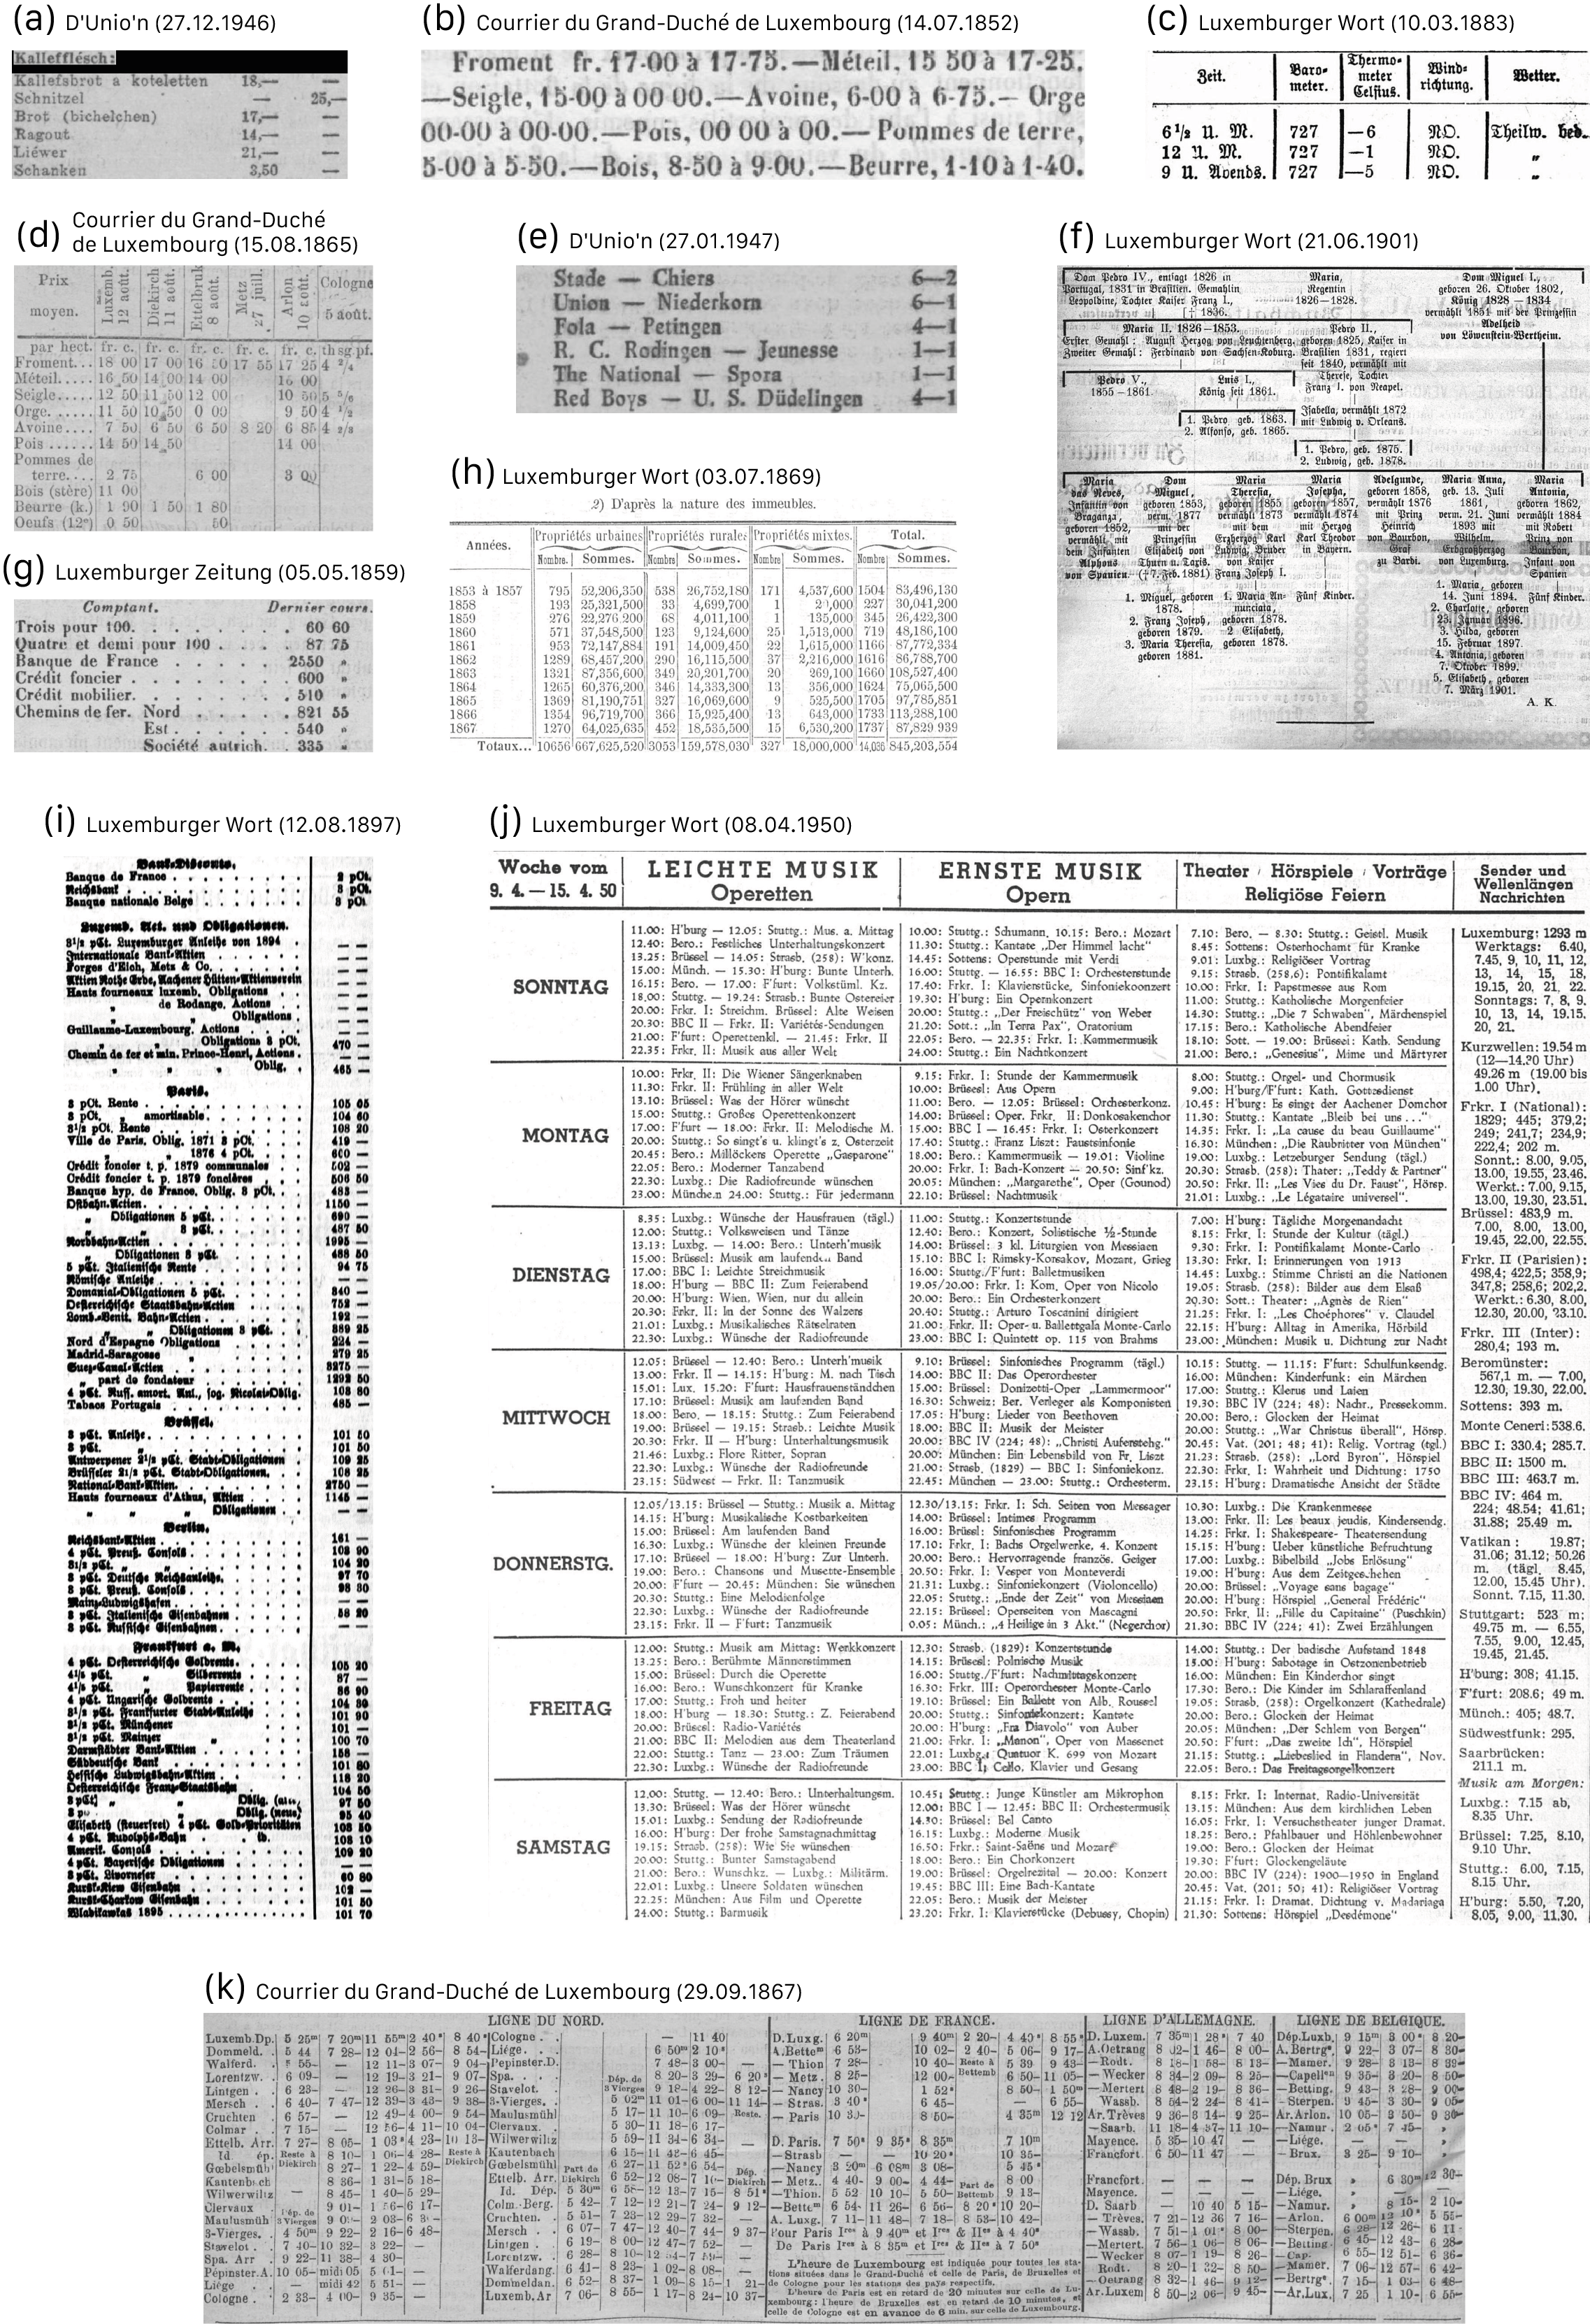
\includegraphics[width=0.95\textwidth]{panel_tables.jpg}
\caption{A panel of tables encountered during the development of the project.}
\label{panel_tables}
\end{figure}

\section{Data sources}
\label{data_sources}
Two different sources were explored to build datasets for table detection and table classification. 

\subsection{Newspaper dataset of the National Library of Luxembourg}
The National Library of Luxembourg, a partner in the \textit{impresso} project, has granted access to its scanned collection of newspapers, which has the particularity of containing segmented portions of the newspaper pages annotated as tables. The data consists of high-resolution scans of Luxembourgish newspapers pages accompanied by rectangular pixel coordinates delineating the locations of the different layout elements on these scans. Segmentation was obtained by applying Optical Layout Recognition (OLR) methods. In addition, an Optical Character Recognition (OCR) was performed and the output is accessible as text tokens with their associated bounding box coordinates. \\
Originally, the dataset was constructed semi-automatically, i.e., tables were detected automatically and then a sample was checked manually. If the number of errors in the sample was within established limits, the overall segmentation was considered correct. Some details on this process are given on a document setting the technical requirements available online.\footnote{\url{https://data.bnl.lu/data/historical-newspapers/}} In summary, five out of every thousand issues were sampled and the maximum number of errors (categorized as blocking, minor or major errors) allowed was set across all types of newspaper items combined. No blocking errors were tolerated, and a maximum of one major and four minor errors were allowed per sixteen pages in a single issue. An exhaustive list of what is considered an error is given in the technical requirements of the library. Unfortunately, this means that it is not possible to draw any solid conclusions about the quality of table annotations of tables in particular. Nevertheless, because of the high standards set by the library, this data provided a seemingly perfect starting point for creating a representative dataset of newspaper tables.\\
As mentioned, OLR was applied to all newspaper pages to identify their constituent elements. These elements are often associated with an instance of a larger layout object. Figure \ref{nll_segmentation_articles} gives an idea of the original segmentation provided by OLR where each color corresponds to one of these instances. For simplicity, we will henceforth refer to these instances as articles or journal items. As can be seen, several bounding boxes can be associated with a single article. Note also that some parts of the page (e.g. the masthead) have not been segmented. Figure \ref{nll_segmentation_tables} shows only the segmentation of articles labelled as table. Note how an instance of a table can also be split in multiple bounding boxes. This is because the titles as well as the sources of the data used in the table (as in the Figure) are often segmented separately from the table itself. The overall segmentation should therefore be taken with a grain of salt, as it may not exactly represent the original segmentation made by the journal editors.

\begin{figure}
\centering
\begin{tabular}{cc}
\subfloat[All types of articles (from Luxemburger Zeitung (10.03.1858), page 1)\label{nll_segmentation_articles}]{\includegraphics[width=0.45\textwidth]{nll_segmentation_articles.png}} &
\subfloat[Tables only (from d'Letzeburger Land (15.05.1987), page 14)\label{nll_segmentation_tables}]{\includegraphics[width=0.45\textwidth]{nll_segmentation_tables.png}}
\end{tabular}
\caption{Original segmentation of newspaper pages coming from the collection of the National Library of Luxembourg.}
\end{figure}

\subsubsection{Statistical exploration}
\label{nll_exploration}
The dataset of the National Library of Luxembourg consists of 58,011 articles labelled as tables distributed across 28,497 pages, themselves spread over 22,735 different newspaper issues. Figure \ref{issue_distribution} shows the distribution of these 22,375 issues with annotated tables over time, relative to the full \textit{impresso} Luxembourg newspaper corpus, which contains 65,515 different issues. This highlights the skewed temporal distribution of the table dataset, where issues appearing before circa 1875 are over-represented. This could generate some bias towards tables that appear only during this period. A similar distribution is observed when comparing the distribution over time of the pages of the table dataset vs. of the full Luxembourg \textit{impresso} corpus (352,137 pages) (Figure \ref{page_distribution}), and the distribution of tables vs. of the 2,372,990 articles (Figure \ref{article_distribution}). It is difficult to draw a conclusion as to whether or not the use of tables in newspapers was more prominent towards the years 1855-1875. However, under the assumption that the number of newspaper issues containing at least one table is stable over the years, Figure \ref{issue_distribution} might indicate that the automatic detection of tables by OLR did not perform equivalently across issues and/or time.  \\

\begin{figure}
\centering
\begin{tabular}{c}
\subfloat[Distribution of the issues\label{issue_distribution}]{\includegraphics[width=0.67\textwidth]{issue_distribution.png}} \\
\subfloat[Distribution of the pages\label{page_distribution}]{\includegraphics[width=0.67\textwidth]{page_distribution.png}} \\
\subfloat[Distribution of the articles\label{article_distribution}]{\includegraphics[width=0.67\textwidth]{article_distribution.png}}\\
\subfloat[Distribution of the average size of tables\label{table_size_normalized}]{\includegraphics[width=0.67\textwidth]{table_size_normalized.png}} \\
\end{tabular}
\caption{Distributions over the years for the data of the National Library of Luxembourg.}
\end{figure}

In order to get additional insights on the legacy OLR from the National Library of Luxembourg for the case of tables, Figure \ref{table_size_normalized} shows the mean and standard deviation of the pixel area (normalized by the page area) tables take in pages that contain at least one table. We see that the average area occupied by tables in pages appears to increase slightly over time. Many interpretations are possible at this point. It could be due to a change in the layout of newspapers, which evolved from very condensed (possibly due to printing costs) to more spaced out through time. It could also point towards inconsistent annotation: assuming that the number of tables is constant over time, it is possible that tables in the later years actually contain multiple tables, thus increasing their average area and diminishing their numbers (as seen in Figure \ref{article_distribution}).\\
Finally, Figure \ref{pages_per_journal} shows the number of pages per title that contain tables, while Figure \ref{pages_per_journal_normalized} compares these values to the total number of pages per journal. Some titles, such as the \textit{Luxemburger Wort} (luxwort), have a lot of pages with tables (24,159) but these pages amount only to a small percentage (2.18\%) of their total pages, while other titles, such as the \textit{Luxemburger Zeitung} (luxzeit1858), are in the opposite situation, i.e., they have a large percentage of their pages that contain tables (13.14\%) but these only amount to a low total number (1,623). This discrepancy in percentages could be explained by the types of articles (perhaps more data-oriented) or the layout of the journal, which makes it easier during OLR to detect the tables.

\begin{figure}
\centering
\begin{tabular}{cc}
\subfloat[Pages with tables\label{pages_per_journal}]{\includegraphics[width=0.45\textwidth]{pages_per_journal.png}} &
\subfloat[Ratio of pages with tables normalized over total number of pages\label{pages_per_journal_normalized}]{\includegraphics[width=0.45\textwidth]{pages_per_journal_normalized.png}}\\
\end{tabular}
\caption{Distributions of the number of pages for each journal.}
\end{figure}

\paragraph{Dataset naming}
In order to facilitate writing and overall understanding, the dataset consisting of all the pages that make up the National Library of Luxembourg collection will now be referred to as \textbf{NLL-full}. The subset of \textbf{NLL-full} consisting solely of pages containing articles labelled as tables will be referred to as \textbf{NLL}.

\subsection{Raphaël Barman's Master project}
\citet{barman_historical_2019} is a Master project previously conducted at the EPFL-DHLAB that explored the ability of a visual model integrating textual clues to segment certain classes of articles in newspapers archives. During this project, a dataset had to be built with manually annotated and tagged articles. The tag set used included \textit{stock exchange tables} that fit exactly what we were looking for. This dataset seemed to be an excellent way to quickly increase the amount of relevant data, while also providing some diversity. Indeed, the dataset was constructed by sampling only from Swiss-French newspapers, which should differ in some way from Luxembourgish newspapers in terms of layout and language. The sampling was done on three journals, the \textit{Journal de Genève} (JDG), \textit{L'Impartial} (IMP) and the \textit{Gazette de Lausanne} (GDL), by randomly taking three issues every 3 or 5 years depending on the journal. Figures \ref{rb_segmentation_tables} and \ref{rb_segmentation_tables2} show some examples from this dataset. The tables have been annotated at the pixel level, which means that an instance of a table can contain multiple tables. Finally, it should be noted that due to the smallness of the dataset, it was quick to verify whether every annotated stock exchange tables were indeed tables: surprisingly, 24 had to be removed. We should point out that it is possible that some tables, which were not stock exchange tables, were not annotated, making this dataset slightly inconsistent. 

\begin{figure}
\centering
\begin{tabular}{cc}
\subfloat[Gazette de Lausanne (15.02.1997), page 19\label{rb_segmentation_tables}]{\includegraphics[width=0.45\textwidth]{rb_segmentation_tables.png}} &
\subfloat[Journal de Genève (23.02.1867), page 3\label{rb_segmentation_tables2}]{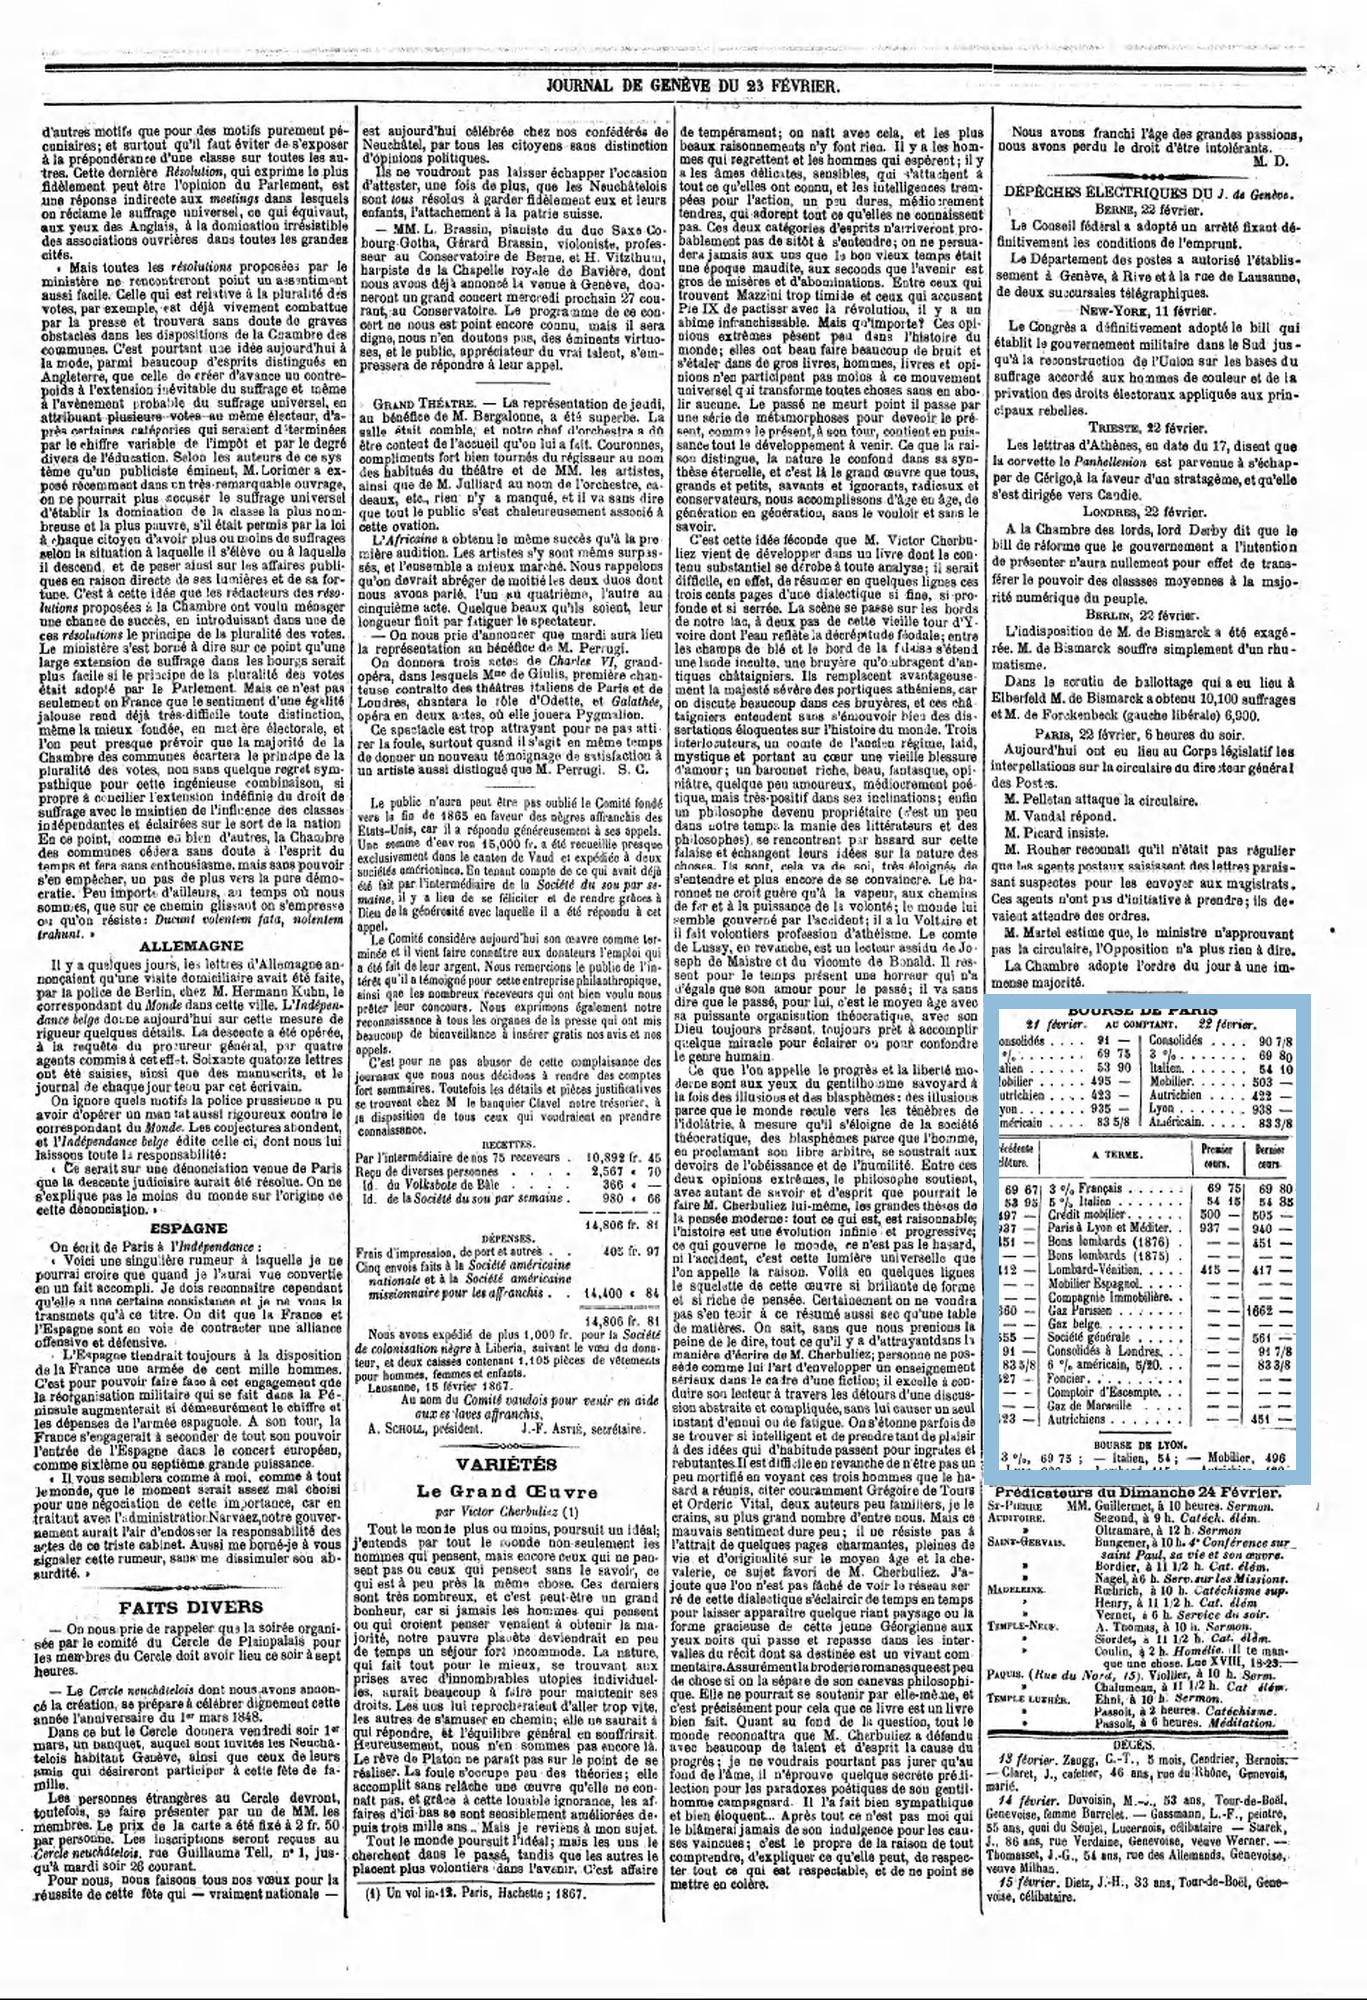
\includegraphics[width=0.45\textwidth]{rb_segmentation_tables2.png}}\\
\end{tabular}
\caption{Original segmentations of newspaper pages coming from \citet{barman_historical_2019}.}
\end{figure}

\subsubsection{Statistical exploration}
In total, the dataset contains 800 tables spread over 474 pages from 3 different titles, themselves spread over 311 issues. Figure \ref{rb_page_distribution} shows the distribution of pages over time for each title. JDG is the most prominent journal because it was sampled every 3 years while the other two were sampled every 5 years. We can notice that stock exchange tables seem to be more numerous between circa 1985 to 1995, with a drop between circa 1915 and 1975.

\begin{figure}[h]
\centering
\includegraphics[width=0.75\textwidth]{rb_page_distribution}
\caption{Distribution over time of the number of pages containing stock exchange tables coming from \citet{barman_historical_2019}.}
\label{rb_page_distribution}
\end{figure}

\paragraph{Dataset naming}
From now on, the dataset containing these 474 pages with stock tables will be referred to as \textbf{RB}.

%\subsection{ICDAR}
%The International Conference on Document Analysis and Recognition (ICDAR) is an academic conference held every two years which proposes competition on different topic centred around %document analysis. In 2019, a competition on Table Detection and Recognition (cTDaR) \cite{gao_icdar_2019} took place in which a large dataset consisting of documents containing all %sorts of tables: printed, handwritten, historical, modern. This dataset was investigated in order to assess the interest in providing out-of-domain examples to the models.

%\paragraph{Dataset naming}
%This dataset will be referred to as \textbf{cTDaR}.

%\section{Data retrieval and infrastructure}
%\label{data_retrieval_and_infrastructure}
%TODO explain the technical challenges  SOLR IFFF S3

\section{Annotation processes}
\label{annotation_processes}
The many annotation processes of \textbf{NLL} undertaken are detailed here in the order they were conducted. Initially, a subset had to be classified in order to tackle the task of table classification. After this initial annotation, a process to increase the size of the already labelled dataset by automatically tagging tables based on the previous manual annotation was explored. After some initial experiments, problems within \textbf{NLL} were revealed and needed to be investigated. The creation of a dataset that attempts to attenuate them based on a statistical exploration is explained, as well as the motivations behind the creation of a final dataset with properly annotated ground truth.

\subsection{Manual classification of tables}
\label{manual_classification_of_tables}
Since one of the goal of the project was to classify tables under finer grained semantic classes, it was decided to dig deeper into \textbf{NLL} through a manual pass in order to tag some tables and identify a typology that could cover all types of tables found in newspapers across time.

\subsubsection{Annotation tool}
In order to alleviate the traditional pains that accompany any annotation process, a web application was developed as a support tool to efficiently browse datasets consistent with this project's case study, i.e., images (tables in this case) cropped out from larger images (newspaper pages in this case). The tool allows the user to increase their tagset as they go through the dataset and discovers new classes. In Figure \ref{letagger}, the application interface can be seen. The left-hand side displays the complete list of tables that can be browsed by category (tagged/untagged/tagged by class), while on the right-hand side are displayed the images similar to the image on the left.\\
Sometimes the legacy segmentations of \textbf{NLL} poorly frame the tables to be tagged; the annotator will then need additional contextual clues to correctly classify the table. In such cases, it becomes necessary to zoom out and look at the entire newspaper page, which is easily achievable with this tool, thus ensuring a qualitative annotation process. In addition, the tool also allows the user to quickly query images that resemble the one they are looking at, provided the dataset meets the infrastructural requirements. This aspect of the tool is discussed in more detail in \ref{automatic_classification_of_tables}.\\

\begin{figure}[h]
\centering
\includegraphics[width=0.9\textwidth]{letagger.png}
\caption{A view of the web application developed to support the annotation processes undertaken during the project.}
\label{letagger}
\end{figure}

\subsubsection{Annotation process}
Using the annotation tool, we needed to create a typology robust enough that it could efficiently summarize \textbf{NLL}. A total of 3,787 tables were manually classified, which amounts to 6.53\% of the tables in \textbf{NLL}. The annotation was done in three different phases. In the first phase, 525 tables were sampled completely at random. We noticed a lack of visual dissimilarity between tables, likely due the skewed temporal distribution (a characteristic problem of \textbf{NLL} raised before), which motivated a revision of the annotation process. Indeed, since most of the sampled tables came from the over-represented periods, many of them were extremely similar, if not identical, tables. Newspapers often use the same tables across multiple issues for recurring topics, such as transport schedules or stock exchanges. Another reason for the decision to revise the process was the need for a robust typology over several years. Indeed, one could hardly come up with a class for radio or television programs if only tables prior to 1900 are sampled. To overcome this problem, and thus better capture the diachronic properties of the domain under study, both visually and semantically, 491 tables were sampled according to the year they originate from, with a probability inversely proportional to the number of tables coming from that year in the dataset. In short, each year had the same probability of being drawn.\\

\paragraph{Established typology}
Through this annotation process, 12 classes were identified. For each of them an example from Figure \ref{panel_tables} is given as well as the number of items classified:
\begin{itemize}
\setlength\itemsep{0em}
\item transport schedule: train and bus timetables (2,301 items, see example (o));
\item sport results: tables that contain sport results, or sport rankings (403 items, see example (e));
\item stock: tables that contain data related to the stock markets (379 items, see examples (g) and (i));
\item food prices: tables that contain the daily food prices, or food advertisements (177 items, see examples (a), (b) and (d));
\item currency rates: tables that contain data related to the current currency rates (65 items, see example (l));
\item election: tables summarizing electoral results (49 items, see example (k));
\item weather: tables that contain weather data (29 items, see example (c));
\item lotto: tables that contain the results of the lotto (8 items, see example (n));
\item cinema: movie timetables (4 items, see example (m));
\item radio: radio programs (3 items, see example (j));
\item miscellaneous: any tables that do not fit one of the above classes (365 items, see example (h));
\item not a table: tables that were wrongly labelled as such (4 items, see example (f)).
\end{itemize}
Each class needed to contain at least 2 tables to be kept. Note that some classes are semantically very close, and thus were merged later when fed to models. However, at this point, they were not and it is only after a statistical analysis that they were merged. During this annotation process, some inconsistencies have started to be noticed. Indeed, some tables are much larger than others because they are sometimes composed of several smaller tables (see example (o)), or they incorporate some of their surrounding (see example (k)).

\begin{figure}[h]
\centering
\includegraphics[width=0.85\textwidth]{nll_tag_year.png}
\caption{Evolution of the number of pages per class for \textbf{NLL-tag}.}
\label{nll_tag_year}
\end{figure}

\subsubsection{Statistical exploration}
Figures \ref{nll_tag_piechart} and \ref{nll_tag_area_piechart} give an idea of the preponderance of each class of tables by looking at their size and at the total pixel area they covered (normalized by the page areas) respectively. It is clear that there is a strong class imbalance, with classes such as transport schedules or stock that are large both in terms of size and surface. \\
Figure \ref{nll_tag_area} shows the size of the pixel area covered by the tables of each class. Looking at stock tables, they represent only 10\% of the total number of tables but cover about 20\% of the total pixel area covered by tables. In Figure \ref{nll_tag_year}, for each class, the number of pages containing at least one table of said class is plotted over time to get an idea of how these labels has evolved. Note how the presence of transport schedule and food price tables disappears over time. Finally, Figure \ref{nll_tag_confusion} shows the percentage of pages where tables of different classes can be found. For example, currency rates tables are found 80\% of the time on the same page as a stock table, proving their close semantics.

\begin{figure}
\centering
     \includegraphics[width=0.8\linewidth]{nll_tag_area}
     \caption{Table pixel areas per class.}
     \label{nll_tag_area}
\end{figure}

\begin{figure}
\centering
     \includegraphics[width=0.9\linewidth]{nll_tag_confusion}
     \caption{Percentage of pages sharing different classes of tables.}
     \label{nll_tag_confusion}
\end{figure}

\paragraph{Dataset naming}
From now on, this dataset composed of 3,787 classified tables will be referred to as \textbf{NLL-tag}.

\begin{figure}
\centering
\begin{tabular}{cc}
\subfloat[\textbf{NLL-tag}: table counts\label{nll_tag_piechart}]{\includegraphics[width=0.4\textwidth]{nll_tag_piechart.png}} &
\subfloat[\textbf{NLL-tag}: table pixel areas\label{nll_tag_area_piechart}]{\includegraphics[width=0.4\textwidth]{nll_tag_area_piechart.png}}\\
\subfloat[\textbf{NLL-auto}: table counts\label{nll_auto_tag_piechart}]{\includegraphics[width=0.4\textwidth]{nll_auto_tag_piechart.png}} &
\subfloat[\textbf{NLL-auto}: table pixel areas\label{nll_auto_tag_area_piechart}]{\includegraphics[width=0.4\textwidth]{nll_auto_tag_area_piechart.png}}\\
\end{tabular}
\caption{Proportions of table counts and total pixel areas in \textbf{NLL-tag} and \textbf{NLL-auto} by class.}
\end{figure}

\subsection{Automatic classification of tables}
\label{automatic_classification_of_tables}
In order to increase the size of \textbf{NLL-tag} with little human effort, an automatic annotation process based on visual similarity was developed. The core idea was to classify all unlabelled tables that are visually similar enough to tables already labelled with the same label. In doing so, the number of tagged tables increased from 3,787 to 8,535. An important point to note when applying this automation is that, even though the number of tagged tables increases dramatically, the number of pages that have all of their tables classified hardly moves at all. Therefore, one should not use this increased dataset by feeding visual models with full pages and expect them to perform efficiently, as the ground truth will be missing a lot of annotations. However, models that only look at tables that have already been segmented can use it. Note that the idea of increasing the size of the dataset using visual similarity may seem a bit odd since it should not bring much diversity to the dataset, but this problem is mitigated if the data is then used for its textual properties for example. Since OCR has been performed on \textbf{NLL-full}, this automatic augmentation makes a lot of sense if this data modality is used for training classifiers.

\subsubsection{Similarity measurement}
The visual similarity comparison was performed using a SOLR\footnote{\url{https://solr.apache.org/}} -- an open-source enterprise-search platform used in \textit{impresso} -- plugin, developed by B. Seguin following his work on visual similarity \citep{seguin_making_2018}, that allows the quick comparison of images whose features vectors have been computed by one of these three visual models: VGG16 \citep{simonyan_very_2015}, Inception-ResNet-v2 \citep{szegedy_inception-v4_2016} and ResNet-50 \citep{he_deep_2015}. The plugin produces a similarity score between 0 and 1 for two images. Two tables were labelled similarly if the following conditions were met: the similarity scores given by the three models were equal to or greater than 0.99, they came from the same titles, there were less than 5 years between their publication. This extremely conservative strategy nevertheless allowed us to increase the dataset size by more than twofold, while generating no errors on a subset of 500 manually checked tables.

\subsubsection{Statistical exploration}
Figures \ref{nll_auto_tag_piechart} and \ref{nll_auto_tag_area_piechart} show the distribution of the number of tables per class and the total pixel areas covered per class. When put to comparison with \textbf{NLL-auto} (Figures \ref{nll_tag_piechart} and \ref{nll_tag_area_piechart}), it can be observed that the class imbalance has increased. This may mean that the classes whose size has increased the most are the most visually stable in \textbf{NLL}. As one might expect, the transport schedules and the stock tables increased the most, as they are often reused as is in sequential newspaper issues.

\paragraph{Dataset naming}
From now on, the dataset composed of 8,535 manually and automatically classified tables will be referred to as \textbf{NLL-auto}.

\subsubsection{Final typology}
Since the under-represented classes did not sufficiently increase in size using automatic tagging, it was decided to keep as part of the final typology the six following classes: \textit{transport schedule}, \textit{sport results}, \textit{food prices}, \textit{exchange}, \textit{weather}, and \textit{miscellaneous}. The stock and currency rate tables were merged into the \textit{exchange} class partly as a result of the observation made in Figure \ref{nll_tag_confusion}, where they tend to always be located close to one another but also because they are semantically close. Every other classes, except \textit{weather}, were added to the \textit{miscellaneous} class. \textit{weather} is a very small class whose tables represent only 0.7\% of the size of \textbf{NLL-tag}, however, since its semantics is quite unique, it has not been merged as it would be interesting to see if the models can learn from so few examples.

\subsection{Investigation of the legacy annotations}
\label{annotation_survey}
After running a first series of experiments on the datasets described before, some issues problems residing in the legacy annotations became apparent. When examining the worst predictions made by the visual models, some tables were detected correctly but were not found in the ground truth. \textbf{NLL}, which was initially considered a gold standard began to reveal some of its weaknesses. In order to address these, an investigation was conducted to assess the recurrence of these problems and potential ways to mitigate them. Two annotators were asked to examine 333 newspapers pages each, and to annotate and classify potentially missing tables. In addition to be classified according to the reduced tag set described earlier, missing tables were to be classified into two additional classes:
\begin{itemize}
\item (A) a table is not annotated and is in the vicinity of other tables with which it shares the same semantic class;
\item (B) a table is not annotated and is alone, i.e., there are no annotated tables next to it that share its semantic class.
\end{itemize}
The annotations were made using VGG annotator \cite{dutta_via_2019}, an open-source web application that allows to easily draw geometrical shapes delimiting annotations on images.

\begin{figure}
\centering
\begin{tabular}{cc}
\subfloat[\textit{L'Union} (13.06.1862), page 1\label{nll_discrepancy_1a}]{\includegraphics[width=0.4\textwidth]{nll_discrepancy_1a.png}} &
\subfloat[\textit{L'Union} (23.07.1862), page 1\label{nll_discrepancy_1b}]{\includegraphics[width=0.4\textwidth]{nll_discrepancy_1b.png}} \\
\subfloat[\textit{Luxemburger Wort} (29.09.1865), page 4\label{nll_discrepancy_2a}]{\includegraphics[width=0.4\textwidth]{nll_discrepancy_2a.png}} &
\subfloat[\textit{Luxemburger Wort} (10.12.1865), page 4\label{nll_discrepancy_2b}]{\includegraphics[width=0.4\textwidth]{nll_discrepancy_2b.png}}
\end{tabular}
\caption{Some inconsistencies in the ground truths of \textbf{NLL}. What is considered as \textit{background} is greyed-out, to better see what is considered as \textit{table}. }
\end{figure}

\subsubsection{Discrepancies in the original annotations}
The main problem that the first experiments revealed was that a large number of tables were missing in the original annotations. Even worse, very similar tables that appear regularly, such as transportation schedules, were sometimes annotated and sometimes not. As can be seen in Figures \ref{nll_discrepancy_1a} and \ref{nll_discrepancy_1b} which show two issues of the same title separated by only a few days, the same tables coming from the top row are inconsistently annotated. In this context, it becomes difficult to expect a model to learn what is a table when it is sometimes annotated as such and sometimes as \textit{background}.
Figures \ref{nll_discrepancy_2a} and \ref{nll_discrepancy_2b} show some of the other issues that arose during the annotation process. The tables are inconsistently annotated with respect to their titles, which are not always included. The same is true for the sources of the table, sometimes listed at its bottom. Another important point to note is that sometimes an instance of an annotated table may actually contain several tables, while sometimes for a similar case, each table is annotated as its own instance. Depending on the algorithms used, this inconsistency in the annotations, sometimes made at the pixel level and sometimes at the instance level, can become a problem. To conclude, this annotation process generated some discord later on between the annotators, as their definition of what a table is did not always align. As explained in \ref{on_the_definition_of_tables}, the definition of tables is not obvious and although no tables were deleted in this process, it did generate discussions that led to more precise guidelines for the next annotation process.

\begin{figure}
\centering
\begin{tabular}{cc}
\subfloat[Count per types of errors\label{survey_boxplots}]{\includegraphics[width=0.49\textwidth]{survey_boxplots.png}} &
\subfloat[Count per types of errors after filtering\label{survey_boxplots_filtered}]{\includegraphics[width=0.49\textwidth]{survey_boxplots_filtered.png}} \\
\subfloat[Count per types of errors per class\label{survey_boxplots_tag}]{\includegraphics[width=0.49\textwidth]{survey_boxplots_tag.png}} &
\subfloat[Count per types of errors per class after filtering\label{survey_boxplots_tag_filtered}]{\includegraphics[width=0.49\textwidth]{survey_boxplots_tag_filtered.png}} \\
\end{tabular}
\begin{tabular}{c}
\subfloat[Count per types of errors per title\label{survey_boxplots_journal}]{\includegraphics[width=1\textwidth]{survey_boxplots_journal.png}} \\
\subfloat[Count per types of errors per title after filtering\label{survey_boxplots_journal_filtered}]{\includegraphics[width=1\textwidth]{survey_boxplots_journal_filtered.png}}
\end{tabular}
\caption{Distributions of the number of missing tables in the original annotations.}
\end{figure}

\subsubsection{Survey statistics}
At this point, the guidelines for annotating were not properly set and although both annotators seemed to prefer to annotate all the tables they encountered as different instances, they did not do so consistently. Therefore, the following statistics should be taken with a grain of salt, although they are sufficient to give an idea of the recurrence of the problems.
Figure \ref{survey_boxplots} shows the number of missing tables found, belonging to class A or B. On average, there are 1.02 missing tables per page, which seems like a large number, but looking at Figure \ref{survey_boxplots_tag}, it appears that the problem is mainly due to missing transport schedule tables.
Now, if we look at Figures \ref{survey_boxplots_journal_total} and \ref{survey_boxplots_journal_mean} which respectively show the average pixel area in percentage tables take in pages that contain at least one table per title, and the same statistics but only for the missing tables, it is clear that some titles are much more affected than others. Figure \ref{survey_boxplots_journal}, which shows the average number of missing tables per title, confirms that there is no strong correlation between the average pixel area of missing tables and the number of missing tables.
Finally, we investigated whether or not these missing tables are related to certain time periods or page numbers; Figures \ref{count_journal_year} and \ref{area_journal_year} explore the former while Figures \ref{count_per_page_lunion} and \ref{area_per_page_lunion} explore the latter. Each point on these scatter plots represents a page of a journal. The latter two plots illustrate the case of a single title (\textit{L'Union}), but similar tables were generated for each title to identify and target the most problematic pages. Notice how page 1 of \textit{L'Union} appears to be missing tables a hundred percent of the time.

\begin{figure}
\centering
\begin{tabular}{cc}
\subfloat[Number of missing tables\label{count_journal_year}]{\includegraphics[width=0.49\textwidth]{count_journal_year.png}} &
\subfloat[Area of the missing tables\label{area_journal_year}]{\includegraphics[width=0.49\textwidth]{area_journal_year.png}}
\end{tabular}
\caption{Distributions of the missing tables per title across time.}
\end{figure}

\begin{figure}
\centering
\begin{tabular}{c}
\subfloat[Number of missing tables per page \label{count_per_page_lunion}]{\includegraphics[width=0.85\textwidth]{count_per_page_lunion.png}} \\
\subfloat[Area of the missing tables per page\label{area_per_page_lunion}]{\includegraphics[width=0.85\textwidth]{area_per_page_lunion.png}}
\end{tabular}
\caption{Distributions of the missing tables for \textit{L'Union} across time.}
\medskip
\small
Problematic clusters of pages are circled in red. On both Figures, we identified similar clusters in \textit{L'Union}: the page 1 for the years 1862-1868 and the page 4 for the years 1869-1871 seems to always be missing tables on the basis of our investigation. Therefore, we removed every first and fourth pages of \textit{L'Union}, during the mentioned time periods, in \textbf{NLL-filtered}.
\end{figure}

\begin{figure}
\centering
\begin{tabular}{c}
\subfloat[Total table area per page\label{survey_boxplots_journal_total}]{\includegraphics[width=0.85\textwidth]{survey_boxplots_journal_total.png}} \\
\subfloat[Total table area per page after filtering\label{survey_boxplots_journal_total_filtered}]{\includegraphics[width=0.85\textwidth]{survey_boxplots_journal_total_filtered.png}} \\
\subfloat[Total missing table area per page\label{survey_boxplots_journal_mean}]{\includegraphics[width=0.85\textwidth]{survey_boxplots_journal_mean.png}} \\
\subfloat[Total missing table area per page after filtering\label{survey_boxplots_journal_mean_filtered}]{\includegraphics[width=0.85\textwidth]{survey_boxplots_journal_mean_filtered.png}}
\end{tabular}
\caption{Distributions of the table pixel areas per title.}
\end{figure}

\subsubsection{Assessment of the estimated quality of the newly created dataset}
Using the above statistics, problematic clusters were identified and filtered out. As noted, some recurring page numbers from specific journals and time periods had large amounts of missing tables or large pixel areas of missing tables, and thus were filtered out from the manually re-annotated sample of \textbf{NLL}. Figures \ref{survey_boxplots_journal_total_filtered} and \ref{survey_boxplots_journal_mean_filtered} show how the average total table pixel area remained relatively stable while the average total pixel area of the missing tables decreased after filtering. Indeed, the total average area occupied by the tables only decreased from 9.21\% to 6.86\%, a reduction of 25.5\%, while the average area of the missing tables dropped from 2.42\% to 0.81\%, a reduction of 66.5\%. In a way, this means that about 2.35\% of the training examples were lost, but in return 1.61\% of the mislabelled (as background) training examples were removed. Since the amount of training data is still very large overall, this decrease is not problematic. However, it is a good idea to remove any training data that might corrupt the learning of the models. Figure \ref{survey_boxplots_filtered} shows how the average number of missing tables decreased, with an average of about 0.32 missing table per page compared to 1.02 originally. Figures \ref{survey_boxplots_tag_filtered} and \ref{survey_boxplots_journal_filtered} show the same statistic but by classes of tables, and by journals.

\subsubsection{Creation of a filtered-out dataset}
Since the filtering strategy used on the manually annotated subset seemed to bear its fruits, it was applied on \textbf{NLL} in order to re-do already carried out experiments and see if better results were obtained. 

\paragraph{Dataset naming}
This new dataset, now containing 28,098 tables and 16,988 pages, will be referred to as \textbf{NLL-filtered}.

\subsection{Creation of an error-free ground truth}
\label{revised_annotations}
After discovering the inherent flaws in the main data source, it was decided to create a small dataset with a manually revised ground truth in order to properly assess the performance of the different models. This supposedly error-free ground truth was performed by three annotators, each annotating 500 different pages. The annotation guidelines, clearer this time, were the followings:
\begin{itemize}
\item Separate large tables that contain smaller tables (usually only pertain to transport schedules).
\item Do not embed the titles of the table but do embed the headers for all tables. The only exception is if there is a pattern in a journal where the titles are always included, try to conform to it.
\item Do not annotate tables that look too much like lists. Indeed, it is common to find tables in the form of lists of items, where each line is a sentence that follows the same logic but with quotation marks on the lines below to repeat the sentences. 
\item Remove table annotations that are not on table items.
\end{itemize}

Even with clearer guidelines, many ambiguous cases were encountered and discussion had to take place to decide how to deal with them. Some examples of these special cases are shown in Figure \ref{panel_unclear}. In Figure \ref{corrections}, the extent to which some of the legacy annotations were problematic is shown.

\begin{figure}[h]
\centering
\includegraphics[width=0.5\textwidth]{panel_unclear.jpg}
\caption{Examples of edge cases encountered during manual annotation of tables.}
\label{panel_unclear}
\medskip
\small
The item at the top as well as the one at the bottom were considered tables, while the three items in the middle were not.
\end{figure}


\begin{figure}
\centering
\begin{tabular}{cc}
\subfloat[Legacy ground truth\label{good_gt}]{\includegraphics[width=0.45\textwidth]{good_gt.png}} &
\subfloat[Revised ground truth\label{bad_gt}]{\includegraphics[width=0.45\textwidth]{bad_gt.png}} \\
\end{tabular}
\caption{Comparison between the original annotations provided by the National Library of Luxembourg, and the revised annotations.}
\label{corrections}
\medskip
\small
These two ground truths show the difference between what is annotated as \textit{background} and as \textit{table}. Nevertheless, the segmentation of tables was done at the instance level (each table was annotated separately). These instances can be easily guessed in these two examples.
\end{figure}

\paragraph{Dataset naming}
This dataset comprised of 1,500 pages will, from now on, be referred to as \textbf{NLL-revised}.

\begin{figure}[h]
\centering
\includegraphics[width=0.75\textwidth]{datasets_summary.png}
\caption{Recap of the creation of \textbf{NLL-tag}, \textbf{NLL-auto}, \textbf{NLL-filtered} and \textbf{NLL-revised}.}
\label{datasets_summary_schema}
\medskip
\small
\textbf{NLL-full} corresponds to the \textit{impresso} Luxembourg corpus, from which \textbf{NLL} was created by taking all pages containing a table. From \textbf{NLL} was created \textbf{NLL-filtered} by applying a filtering strategy to discard pages with an estimated high number of missing tables, \textbf{NLL-tag} by manually tagging some tables, and \textbf{NLL-revised} by revising a subset of it by fixing its annotations. \textbf{NLL-auto} was created by querying \textbf{NLL} to automatically find tables visually similar to those in \textbf{NLL-tag}. 
\end{figure}

\section{Summary}
\label{datasets_summary}
We provide a summary of all the datasets created throughout this project in Table \ref{datasets_distributions}. Each dataset is summarized by their number of table annotations (by class), the number of pages they contain and the number of issues they cover. In Figure \ref{datasets_summary_schema}, we recapitulate how each of these datasets (but \textbf{RB}) were constructed. Note that the size of the datasets may differ slightly from what was reported in the previous sections, because during their creation and subsequent investigations, some mislabelled tables were removed.

\begin{table}[htp]
\begin{center}
\begin{tabular}{c||c|c|c|}
Dataset name & Articles & Pages & Issues \\
\hline
\textbf{NLL} & \begin{tabular}{@{}wl{3.25cm}wr{1cm}@{}}tables & 58,007 \end{tabular} & 28,496 & 22,734\\
\hline
\textbf{NLL-tag} & \begin{tabular}{@{}wl{3.25cm}wr{1cm}@{}}exchange & 444\\food prices & 177\\miscellaneous & 429\\sport results & 403\\transport schedules & 2,301\\weather & 29 \\ \hline tables & 3,783 \end{tabular}& \begin{tabular}{@{}c@{}}312 \\ 143 \\ 237 \\ 41 \\ 408 \\ 28 \\ \hline 984  \end{tabular} & \begin{tabular}{@{}c@{}}312 \\ 143  \\ 228 \\ 41 \\ 407\\ 28 \\ \hline 972  \end{tabular}\\
\hline
\textbf{NLL-auto} &  \begin{tabular}{@{}wl{3.25cm}wr{1cm}@{}}exchange & 1,123\\food prices & 616\\miscellaneous & 461\\sport results & 428\\transport schedules & 5,868\\weather & 35 \\ \hline tables & 8,531 \end{tabular}& \begin{tabular}{@{}c@{}}874 \\ 569  \\ 267 \\ 58 \\ 3062 \\34\\ \hline 4616  \end{tabular} & \begin{tabular}{@{}c@{}}875 \\ 569  \\ 258 \\ 58 \\ 3,060\\34 \\ \hline 4,565  \end{tabular}\\
\hline
\textbf{NLL-filtered} & \begin{tabular}{@{}wl{3.25cm}wr{1cm}@{}}tables & 28,094 \end{tabular} & 16,987  & 15,968\\
\hline
\textbf{NLL-revised} & \begin{tabular}{@{}wl{3.25cm}wr{1cm}@{}}tables & 5,445 \end{tabular} & 1,500  & 1,479\\
\hline
\hline
\textbf{RB} & \begin{tabular}{@{}wl{3.25cm}wr{1cm}@{}}tables & 800 \end{tabular} & 474  & 311\\
\hline
\end{tabular}
\end{center}
\caption{Number of tables, pages and issues per datasets.}
\label{datasets_distributions}
\end{table}%

\chapter{Models and Evaluation}
\label{models}
This chapter expands on two of the main goals of the project: table detection in \ref{table_detection} and table classification in \ref{table_classification}. Each section reviews the models explored to meet these intents and the evaluation of the proposed solutions.

\section{Table detection}
\label{table_detection}
The task of table detection as addressed in this project is to detect and segment tables in newspapers pages. More formally, given an image of a scan of a newspaper page, the goal is to produce one or many segmentation masks that contain tables. Two image segmentation methods were used and compared to get a better idea of how best tackle the table detection problem. Even though these methods follow different image segmentation paradigms, they are both able to provide satisfactory solutions.

\subsection{dhSegment}
dhSegment \citep{ares_oliveira_dhsegment_2018} is a semantic image segmentation algorithm developed at the EPFL-DHLAB, which aims at providing a generic tool for historical document processing. Based on a U-Net architecture \citep{ronneberger_u-net_2015}, but incorporating a residual network as the encoder, it provides pixel-wise probability maps for each class to be detected. This model has already proven its effectiveness, especially in \citet{barman_combining_2021}, where it has shown encouraging results on newspaper pages. Note that all experiments were actually performed using dhSegment-torch\footnote{\url{https://github.com/dhlab-epfl/dhSegment-torch}}, a PyTorch reimplementation of the original model.

\paragraph{Semantic image segmentation}
We recall the definition of semantic image segmentation in the context of table detection. Semantic segmentation refers to the task of predicting the semantic class to which each pixel in an image belongs. In the table recognition use case, each pixel of the image must be defined as belonging either to the \textit{background} or to a \textit{table}. A segmentation mask for tables can then be produced. \\
One of the advantages of semantic segmentation is that the training material can be annotated at a coarse granularity: tables do not need to be individually annotated since they do not need to be individually detected. However, this makes the task of table classification very difficult, because it has to deal with a segmentation mask that may cover several tables from different classes, even when considering the different connected components (separate clusters of pixels) of the mask separately.

\paragraph{Model}
In this project, the architecture of dhSegment uses a ResNet-50 \citep{he_deep_2015} pre-trained on the ImageNet dataset \citep{deng_imagenet_2009} as its encoder. It uses the default implementation of dhSegment as described in the original paper, which limits the number of features channels in the expanding path to 512 for memory reasons.

\paragraph{Training}
The training hyper-parameters are detailed later for each experiment, as they vary slightly. However, what remains constant is the use of the mean intersection over union (mIoU) metric (see Section \ref{table_detection_evaluation}) to guide the training of the network.

\paragraph{Inference}
For the task of table detection, the network is asked to output two probability maps that indicate the likeliness each pixel is part of the \textit{background} or part of a \textit{table}. A prediction map is then created from these two probability maps, where each pixel is assigned to the most probable class. Finally, the connected components that represent less than 0.5\% of the page are removed, in agreement with the methodology proposed in \cite{barman_historical_2019}. In Figure \ref{inference_dhsegment}, a complete example is shown where the leftmost image corresponds to a ground truth, with tables annotated in a lighter colour; the middle image shows the probability map for the table class; and the rightmost image shows the final prediction. The spot on the left of the probability map is not part of the final prediction because the network has determined it as more likely to be part of the background. 

\begin{figure}
\centering
\begin{tabular}{ccc}
\subfloat[Ground truth]{\includegraphics[width=0.30\textwidth]{gt_dhsegment.png}} &
\subfloat[Probability map for tables]{\includegraphics[width=0.30\textwidth]{prob_dhsegment.png}} & 
\subfloat[Prediction map]{\includegraphics[width=0.30\textwidth]{pred_dhsegment.png}}\\
\end{tabular}
\caption{Inference process of dhSegment.}
\label{inference_dhsegment}
\end{figure}

\subsection{Mask R-CNN}
Mask R-CNN \citep{he_mask_2018} is an object instance image segmentation algorithm, originally developed at Facebook AI Research and commonly used for its versatility, which has shown good results for document image analysis. Built after the Faster R-CNN architecture \citep{ren_faster_2016}, it follows the same two-stage procedure with slight improvements. First, feature maps are generated for the image using a feature extractor network, that is referred as the \textit{backbone}. These are passed through a region proposal network (RPN) that detects regions of interest (RoI). Second, visual features are extracted and pooled from the image feature maps for each RoI using an operation called RoIAlign. RoIAlign ensures that the extracted sub-maps for each RoI have the same dimensions and are not affected by quantization problems induced by dimension changes. The feature sub-maps of each RoI finally pass through the \textit{head} of the backbone and an added branch for mask segmentation. A label, bounding box coordinates and a segmentation mask (at the pixel level) within the bounding box are finally output for each RoI. Note that ResNet models \citep{he_deep_2015} are generally the preferred choice for the backbone, and that its head refers to the final layers used for prediction, which will differ for each model.\\
The implementation of Mask R-CNN used in this project comes from the MMDetection library \citep{chen_mmdetection_2019}, an open-source toolbox for image detection tasks.

\paragraph{Object instance image segmentation}
We recall the definition of object instance image segmentation and complete it according to our specific case. Object instance segmentation consists in detecting clusters of pixels belonging to the same semantic class while identifying each instance of that class separately. It therefore requires fine-grained ground truth annotations, as each table must be distinctly annotated for models to understand they are different instances of the same semantic class. It differs from semantic image segmentation in that regard.\\
When talking about object instance image \textit{detection}, as opposed to object instance image \textit{segmentation}, the goal is only to detect objects (with a bounding box) and not to actually segment them. Because these tasks are so popular, they have their share of conventional formats associated with them for annotations. COCO \citep{lin_microsoft_2014} being one of them, it was used in this project and is briefly described below.

\paragraph{COCO}
Common Objects in Context (COCO) is originally a dataset compiled by Microsoft that contains a large amount of images representing complex scenes of everyday life annotated according to an annotation format they proposed. This format is now widely used for object instance detection tasks and had to be used here in order to feed the data to the MMDetection library. \\
COCO also refers to a series of competitions around image detection tasks\footnote{\url{https://cocodataset.org/\#detection-eval}} in which many metrics have been chosen to compare the performance of models and have become standards in the field. These metrics are explained later in \ref{table_detection_evaluation}.

\paragraph{Model}
The architecture of the Mask R-CNN model used in this project is somewhat similar to that of dhSegment, as the backbone of its convolutional architecture is also a ResNet-50. However, it is also coupled with a Feature Pyramid Network (FPN) \citep{lin_feature_2017} that helps extract better features from the RoI by compiling in a top-down manner the feature maps generated by the backbone. The model was pretrained on the ImageNet dataset for 36 epochs. 

\paragraph{Training}
The training hyper-parameters are detailed later, as they vary from experiment to experiment. However, what remains constant is the use of the mean average precision (mAP) metric (see Section \ref{table_detection_evaluation}), on the segmentation masks, to guide the training of the network. Indeed, the mAP can be computed either based on the segmentation masks of each proposed instance by the model or on their bounding boxes. Since tables are not always rectangular, we force the network to learn on the segmentation masks. Therefore, each evaluation metric reported in this thesis for Mask R-CNN are computed using these. 

\paragraph{Inference}
The model outputs the bounding box coordinates of each of the detected instances, as well as a segmentation mask within these bounding boxes along with a confidence score ranging from 0.05 to 1 for each instance. An example is shown in Figure \ref{example_mask}, where the ground truth of each table instance is shown in blue, and each prediction is shown as a red bounding box and a segmentation mask inside. The confidence score and class of each prediction is marked at its top.

\begin{figure}
\centering
\begin{tabular}{cc}
\subfloat[Ground truths (blue) and object instance predictions (red)\label{example_mask}]{\includegraphics[width=0.45\textwidth]{pred_mask.png}} &
\subfloat[Semantic prediction\label{prediction_mask}]{\includegraphics[width=0.45\textwidth]{semantic_mask.png}} \\
\end{tabular}
\caption{Comparison between Mask R-CNN object instance and semantic predictions.}
\label{inference_mask}
\end{figure}

\subsection{Evaluation}
\label{table_detection_evaluation}
Semantic image segmentation and object instance image segmentation are two tasks that each have well-established sets of metrics used to evaluate models. Some of these metrics are presented here, starting with the Intersection over Union (IoU) used for semantic segmentation. Next, the Average Precision (AP), a widely used metric for object instance image segmentation tasks and the primary metric for COCO challenges, is explained. Finally, the relationship between these metrics is explained, as well as a strategy for effectively comparing semantic and object instance segmentation models.

\subsubsection{IoU (Intersection over Union)}
The IoU measures the quality of a predicted segmentation mask by computing its intersection with the corresponding ground truth segmentation mask over their union. Formally, if P is the set of predicted pixels and G the set of pixels belonging to the ground truth, IoU is defined as follows:
\[ IoU(P,G) = \frac{|P \cap G|}{|P \cup G|} \]
Often, this metric is computed for every images and every classes to be detected and then averaged. It is referred to as the mean Intersection over Union (mIoU). If $P$ is the set of all predictions, $G$ is the set of all ground truths, $P_{i,c}$ is the set of pixels predicted for image $i$ and class $c$, $G_{i,c}$ the set of pixels that belongs to the ground truth for image $i$ and class $c$, $I$ is the set of images, $C$ is the set of classes, and $I_{c} = \{i \in I : | P_{i,c} \cup G_{i,c}| > 0\}$, then the mIoU is computed as follows:
\[ mIoU(P,G) =\frac{1}{|C|}\frac{1}{|I|} \sum_{i \in I, c \in C}IoU(P_{i,c}, G_{i,c}) \]
Note that the mIoU can also be computed on a per-class basis in order to assess the quality of a model on each class individually, by having only one class in $C$. \\

\subsubsection{AP (Average Precision)}
\label{ap}
AP corresponds to the area under the Precision-Recall curve.

\paragraph{Precision-Recall curve}
The Precision-Recall curve is a function that maps recall to precision for a given model on a specific class. As a reminder, precision is an empirical evaluation measure of a model's ability to make predictions that match ground truths, while recall is an empirical evaluation measure of a model's ability to predict all ground truths. Formally, if TP stands for the number of true positives, TN for true negatives, FP for false positives and FN for false negatives, they are defined as follows:
\[ \text{Precision} = \frac{TP}{TP + FP} \]
\[ \text{Recall} = \frac{TP}{TP + FN} \]
When computing the precision for a certain recall, predictions are sorted by their confidence level and only the first predictions necessary for the model to reach the given recall are considered in the computation of the precision. Since the range of values the recall can take is finite, values between two consecutive points are interpolated by linking these two points. \\
Different strategies are then taken to compute the area under the curve. Generally, a set of evenly spaced recall levels is determined and precision is computed for these recalls. Since a specific recall may not exist for a given solution, the precision for this specific recall value becomes the maximum precision for every recall values larger than the one considered. When computing the AP for the COCO challenge, the set of considered recalls corresponds to $\{0.01*x : x \in \mathbb{Z}_{[0, 100]} \}$, i.e. a set of 101 evenly spaced recall values. In this project this definition is used when computing the AP. \\
Often, this metric is computed for every classes to be detected and then averaged. It is then referred to as mean Average Precision (mAP), even though sometimes also loosely referred to directly as AP. 

\subsubsection{IoU as a threshold}
The IoU is often used to determine whether a prediction should be considered correct or not. It can then be used in conjunction with more traditional metrics such as precision and recall in image segmentation algorithms. The methods for computing precision and recall for semantic image segmentation algorithms and object instance image segmentation algorithms are similar in their use of the IoU to determine the correctness of a prediction, but differ in the amount of predictions made per image.\\
Semantic image segmentation algorithms produces a single mask per image and per class. To assess the correctness of a solution, the following methodology is used. When the IoU between a prediction and a ground truth is above a threshold $\tau$, the prediction is considered a true positive (TP). When $0 < IoU < \tau$, the prediction is considered as a false positive (FP). When no prediction is made and the union is equal to 0, the prediction is considered a true negative (TN). Finally, when $IoU = 0$ and the size of the ground truth is larger than 0, the prediction is considered a false negative (FN). Therefore, the precision and the recall of a semantic segmentation model can be computed, but works on a page level and therefore it is not possible to know exactly how many tables were detected.\\
Object instance image segmentation algorithms make many predictions per image and per class. In this paradigm, to assess the quality of a solution, a similar methodology is followed. The same logic is followed for TP, FP and FN. However, TNs are not considered as there could be infinitely many instances of bounding boxes that should not be detected on a page. Since TNs are not considered in the computation of precision and recall, it is not an issue. Another important aspect to point out is that when multiple predictions are made for a same ground truth object, only the one with the largest IoU is counted as a TP while the others are counted as FP. \\
With this in mind, it becomes clear that precision and recall must be computed by setting a threshold on the IoU beforehand. Precision is then referred to as Precision at $\tau$ or P@$\tau$, and recall follows the same logic. Note that it is also possible to average a metric over multiple IoU thresholds as well. One may want to average precision over IoU values ranging from $\tau_{start}$ to $\tau_{end}$ with a step of $\tau_{step}$, this would be written as P@$\tau_{start}$:$\tau_{step}$:$\tau_{end}$. The same logic follows for recall. Finally, note that since (m)AP relies on precision, recall and thus on the IoU, it also follows the same notation logic.

\subsubsection{Comparing semantic and object instance image segmentation algorithms}
As explained, semantic image segmentation algorithms and object instance image segmentation algorithms are difficult to compare because the numbers of TPs, FPs, TNs and FNs may largely differ. A simple solution is proposed in this project by interpreting the solution produced by the latter class of algorithms as if it had been output by a semantic image segmentation algorithm. To do so, the segmentation masks of each object instance proposed by the algorithm are considered as if they were the result of a single prediction and are thus merged into a single segmentation mask per image. Thus, it is now possible to compute the mIoU at the page-level as it is the case for semantic image segmentation algorithms. An example can be seen in Figure \ref{prediction_mask}, where the original output of Mask R-CNN seen on the left figure is modified as explained. Note that, as explained earlier, the predictions of Mask R-CNN all have a confidence score, starting from 0.05, associated with them. In the methodology we propose here all predictions with a score greater or equal to 0.05 are considered and turned into a semantic mask.

\section{Table classification}
\label{table_classification}
Table classification, in the context of this thesis, refers to the task of classifying tables found in newspaper pages. More formally, given an image that corresponds to a table segment from a scan of a newspaper page, as well as its OCR (text tokens and their bounding box coordinates), the goal is to classify said table using a given label set. Three models using different combinations of data modalities, including text, layout information and images, were used and compared on this task.

\subsection{RoBERTa}
RoBERTa \citep{liu_roberta_2019} is a language representation model based on BERT \citep{devlin_bert_2019}, which stands for Bidirectional Encoder Representations from Transformers. BERT is based on the encoder part of the Transformer architecture \citep{vaswani_attention_2017}, which used two novel strategies for its pre-training. First, the use of masked language modelling, where words in sentences are randomly masked and the network is asked to guess them. Second, the task of next sentence prediction, where the network must guess whether two given sentences have been written next to each other, was created. In order for the model to be able to handle this latter task, BERT also improves on the input representation by allowing for an arbitrary span of contiguous text. Input sentences, in the context of BERT, can therefore be arbitrarily long and contain multiple sentences or a complete document. These strategies contributed in making BERT a state-of-the-art model for many language understanding tasks. Note there exist two versions of BERT consisting of differently sized Transformers architecture: the BASE model contains 110M parameters, while the LARGE model contains 340M parameters. Still, RoBERTa is able to improve on BERT by revising its pre-training, essentially increasing the amount of data used for training, changing some key hyper-parameters used in the training setup, and by removing the next sentence prediction task. RoBERTa stands for Robustly optimized BERT approach. RoBERTa is thus a standard language representation model that takes only text as input and can classify it when a sentence (in the BERT sense) classification head, i.e. a linear layer, is connected to the end of the network. 

\paragraph{Model}
The model used in this project is actually a multilingual version of RoBERTa dubbed XLM-RoBERTa \citep{conneau_unsupervised_2020}, that was trained on one hundred different languages. It is motivated by the fact that the newspapers used in this project are written in different languages: French, German and Luxembourgish. The BASE version is used for memory reasons, with a maximum sequence length of 512 tokens.\\
The implementation of the model comes from the transformers library \citep{wolf_huggingfaces_2020}, a large online library of pre-trained machine-learning models. 

\paragraph{Training}
The training is done following the default hyper-parameters proposed by the library in its version 4.14.1 The accuracy of the model on its validation set is the metric chosen to guide its training.

\paragraph{Inference}
The network outputs logits for each class and the class with the largest one is chosen as the prediction.

\subsection{LayoutLM}
\label{layoutlm}
LayoutLM \citep{xu_layoutlm_2019} is a model for document image understanding and information extraction tasks that modifies the original BERT architecture by incorporating additional layout and image information. Each word token is concatenated with an embedding of its bounding box coordinates and a visual embedding of the image region given by its coordinates. In addition to this, a visual embedding of the entire document image is also concatenated. These visual embeddings are produced by Faster R-CNN \citep{ren_faster_2016}.\\
Although this model can use the visual modality, it was not used in this project. In the original paper, this modality was not used during pre-training and was to be used only for fine-tuning. But a second version of the model called LayoutLMv2 \citep{xu_layoutlmv2_2021} was introduced later and used it during pre-training. This new model is therefore better adapted to evaluate the added value of this modality: this model is introduced afterwards in \ref{layoutxlm}. 

\paragraph{Model}
LayoutLM BASE model was used, which is built over BERT BASE model, and is therefore of similar size. Input sequences must be of length 512. The implementation of LayoutLM also comes from the transformers library; note that it lacks a straight-forward way to make use of the visual data.

\paragraph{Training}
The training is done following the default hyper-parameters proposed by the library in its version 4.14.1 The accuracy of the model on its validation set is the metric chosen to guide its training.

\paragraph{Inference}
Trivially, the class with the largest logit is chosen as the prediction.

\subsection{LayoutXLM}
\label{layoutxlm}
LayoutXLM \citep{xu_layoutxlm_2021} is a multilingual extension of LayoutLMv2 \citep{xu_layoutlmv2_2021} trained on 53 languages; the latter is an improved version of the aforementioned LayoutLM where the only difference is the use of the visual modality during its pre-training making it more efficient. 

\paragraph{Model}
LayoutXLM BASE model was used, which is built over BERT BASE model, and is therefore of similar size. It expects input sequences of length 512. The implementation of LayoutXLM also comes from the transformers library.

\paragraph{Training}
Unlike the training of LayoutLM, the visual modality was used when fine-tuning this model. The training is performed following the default hyper-parameters proposed by the library in its version 4.14.1. The accuracy of the model on its validation set is the metric chosen to guide its learning.

\paragraph{Inference}
The class with the largest logit is chosen as the prediction.

\subsection{Evaluation}
\label{table_classification_evaluation}
When it comes to evaluating the quality of a classifier, precision and recall are commonly used and have already been defined in \ref{ap}. Accuracy is also often used, it measures the proportion of correct predictions made by a model and can be defined as follows:
\[ \text{Accuracy}=\frac{TP + TN}{TP + TN + FP + FN}\]
Finally, another important metric is the F1-score, which can be defined as the harmonic mean of the precision and recall. More formally,
\[ \text{F1-score}=2*\frac{Precision * Recall}{Precision + Recall}\]
Since the problem at hands requires classifying objects into several classes, which may be largely unbalanced and thus strongly bias the above mentioned metrics, it is interesting to run these metrics separately on each class. Another tool to better visualize the results obtained is the confusion matrix which integrates the number of good and bad predictions for each class and allows to easily see which classes are confused by the classifier.

\chapter{Experiments}
\label{experiments}
This chapter covers the different experiments conducted in the context of this project. In Section \ref{experiments_table_detection}, we present two experiments on table detection, which investigate the ability of image segmentation models to learn under challenging data condition. Two experiments on table classification are also presented in Section \ref{experiments_table_classification}, where we examine the predictive power of state-of-the-art classifiers using different data modalities on manually and automatically constructed datasets. Finally, in Section \ref{end_to_end}, we present an inconclusive experiment conducted at the beginning of this project that shows the difficulty for image segmentation models to simultaneously solve the tasks of table detection and table classification.

\section{Table detection}
\label{experiments_table_detection}
In Section \ref{table_detection_experiment1}, the performances of dhSegment and Mask R-CNN are compared on datasets with different levels of inconsistencies. In Section \ref{table_detection_experiment2}, these models are compared on a reduced but supposedly perfect dataset.

\subsection{Assessment of a data filtering strategy}
\label{table_detection_experiment1}
Having high quality data is essential to the optimal learning of any machine learning models, but what if the only data available is not? In this experiment, we assess the usefulness of the filtering strategy described in \ref{annotation_survey} -- where problematic clusters are manually identified and removed -- from which \textbf{NLL-filtered} was created out of \textbf{NLL}. Since both datasets are known for being inconsistent, a question that is naturally brought up is whether or not the chosen models are able to learn despite this. To answer it, dhSegment and Mask R-CNN are trained on the two aforementioned datasets and their performances compared on manually constructed datasets.\\
This experiment also serves the purpose of establishing whether object instance image segmentation algorithms are capable of performing semantic image segmentation efficiently, as touched in \ref{table_detection_evaluation}.

\subsubsection{Training}
Models are trained using two different setups summarized in Tables \ref{setup1} and \ref{setup2}. In the first setup, models are trained on \textbf{NLL} using 70\% of the pages for training and 20\% for validation. They are then tested on the remaining 10\%, on \textbf{RB} and on \textbf{NLL-revised}. The second setup is very similar, but models are instead trained (and tested) on \textbf{NLL-filtered} following the same splits.\\
Note that for both setups, \textbf{NLL-revised} only contains pages that are part of the testing splits of \textbf{NLL} and \textbf{NLL-filtered} which ensures that models have not seen these test examples during their training. Finally, we recall that \textbf{RB} has not been annotated at the instance-level, so its evaluation by object instance segmentation metrics should be poor.\\
The different hyper-parameters used for training each model are introduced below. Their search was done by trial and error; they may not lead to the lowest training times but should ensure convergence. This is also the case for the next experiment.

dhSegment and Mask R-CNN were both trained similarly. Their training was done with a batch size of 2 for 25 epochs using batch normalization on a NVIDIA GeForce GTX TITAN X 12GB. An Adam optimizer with an initial learning rate of $10^{-4}$ coupled with a per-epoch exponentially decaying learning rate $\gamma=0.85$ and a L2-regularizer of $10^{-6}$ were used. Both models were pre-trained on the ImageNet dataset. The only difference between both models is their metric to optimize on the validation set, which is the mIoU or dhSegment and the mask segmentation mAP for Mask R-CNN. \\
During training, images are resized to reach an height of 1333 pixels and a width of 800 pixels. After that they are uniformly scaled by a factor randomly sampled from [0.9, 1.1]; the images are cropped to maintain their size. Then, they are slightly rotated 50\% of the time by a degree sampled uniformly from [-1, 1].  \\

For both models, only one run was performed as the training time is very long: about three days for dhSegment, and about two days for Mask R-CNN.

\begin{table}[htp]
\begin{center}
\begin{tabular}{c|c|c||c}
 & Training & Validation & Testing \\
\hline
\textbf{NLL} & \begin{tabular}{@{}c@{}}40,435 tables \\ 19,947 pages (70\%)\end{tabular} &  \begin{tabular}{@{}c@{}}11,706 tables \\ 5,700 pages (20\%)\end{tabular} & \begin{tabular}{@{}c@{}}5,866 tables \\ 2,849 pages (10\%)\end{tabular}\\
\hline
\textbf{RB} &  &  & \begin{tabular}{@{}c@{}}800 tables \\ 474 pages (100\%)\end{tabular}\\
\hline
\textbf{NLL-revised} &  &  & \begin{tabular}{@{}c@{}}5,445 tables \\ 1,500 pages (100\%)\end{tabular}\\
\hline
\end{tabular}
\end{center}
\caption{Table detection, setup 1: datasets splits.}
\label{setup1}
\end{table}%

\begin{table}[htp]
\begin{center}
\begin{tabular}{c|c|c||c}
 & Training & Validation & Testing \\
\hline
\textbf{NLL-filtered} & \begin{tabular}{@{}c@{}}19,641 tables \\ 11,890 pages (70\%)\end{tabular} &  \begin{tabular}{@{}c@{}}5,640 tables \\ 3,399 pages (20\%)\end{tabular} & \begin{tabular}{@{}c@{}}2,813 tables \\ 1,698 pages (10\%)\end{tabular}\\
\hline
\textbf{RB} &  &  & \begin{tabular}{@{}c@{}}800 tables \\ 474 pages (100\%)\end{tabular}\\
\hline
\textbf{NLL-revised} &  &  & \begin{tabular}{@{}c@{}}5,445 tables \\ 1,500 pages (100\%)\end{tabular}\\
\hline
\end{tabular}
\end{center}
\caption{Table detection, setup 2: datasets splits.}
\label{setup2}
\end{table}%

\subsubsection{Results}
Results for the first setup, where models are trained on the large but highly inconsistent \textbf{NLL}, are shown in Table \ref{setup1_results}, while results for the second setup, where models are trained on the medium-sized but mildly inconsistent \textbf{NLL-filtered}, are shown in Table \ref{setup2_results}. \\
In both setups, when evaluated on \textbf{NLL-revised}, Mask R-CNN outperforms dhSegment on all metrics. This means that Mask R-CNN is better than dhSegment at semantically detecting tables on newspaper pages when trained with inconsistent data. We believe that this may be due in part to the fact that Mask R-CNN considers every predictions with a confidence score greater than 0.05 it makes. This means that even if Mask R-CNN thinks a Region of Interest has only 5\% chance of being a table, it will be part of its prediction. As in most object instance image segmentation algorithms, low-certainty predictions are not discarded assuming that they can be filtered later based on the overall Precision-Recall ratio one is interested in. This explanation seems to be corroborated by \citet{wenkel_confidence_2021} who state that, in the context of object detection algorithms, ``most neural networks use a rather low threshold as a high number of false positives is not penalized by standard evaluation metrics''. Indeed, this strategy would therefore not be penalized on \textbf{NLL-revised} since it contains many more tables than \textbf{NLL}. False positives in the latter dataset appear to result in true positives in the former. The large APs of Mask R-CNN on both \textbf{NLL} and \textbf{NLL-filtered} also point in that direction, as the model is perfectly capable of performing well on a testing dataset representative of its training: a large number of false positives is indeed not penalized by standard evaluation metrics for object detection.  \\
Looking at the results of both models for both setups on the test sets of the data they were trained with, we find that dhSegment generally outperforms Mask R-CNN on all metrics except mIoU and R@50:5:95 for \textbf{NLL}. We should also point out the notable increase in mIoU for dhSegment between both datasets when trained with the more consistent dataset \textbf{NLL-filtered} compared to \textbf{NLL}. Overall, this suggests that dhSegment is better than Mask R-CNN when tested on data representative of that on which it was trained on, and that when the data is more consistent, it is able to achieve better performance on semantic segmentation metrics. It is true that Mask R-CNN also sees a performance increase on the mIoU, but it is smaller than that of dhSegment (+0.48 vs +1.65 on the mIoU). We can therefore conclude that the filtering strategy is favorable to dhSegment. Indeed, its performance in terms of mIoU on \textbf{NLL-revised} increases by 5.82 between the two setups, while those of Mask R-CNN decrease by 1.05. Mask R-CNN suffered from the filtering strategy; because of it, it was subjected to less tables, and even if these are known to be inconsistently labelled, Mask R-CNN is able to learn from them. This is also confirmed by its APs which decrease by 0.35 between both setups. \\
In both setups, for dhSegment, we notice a large drop in Precision between the \textbf{NLL} and \textbf{NLL-filtered} test sets and \textbf{NLL-revised}, but a small drop in Recall. Since both \textbf{NLL} and \textbf{NLL-filtered} test sets lack some tables in their ground truth compared to \textbf{NLL-revised}, it is more difficult for the models to reach the IoU threshold that will turn a prediction into a true positive instead of a false positive. As a result, the number of false positives increases and the number of true positives decreases, greatly reducing the Precision. Concerning the Recall, both test sets contain tables that incorrectly labelled as such, which is not the case in \textbf{NLL-revised}. It is likely that dhSegment correctly guessed that certain tables were actually not tables, which was initially penalized due to erroneous ground truth in the test sets but encouraged in \textbf{NLL-revised}. As a result, the number of false negatives decreased, which had less of an impact on the overall decrease in Recall.\\
For \textbf{RB}, we again see a clear advantage on non-representative datasets for Mask R-CNN on all metrics. Also noteworthy are the extremely low AP scores for Mask R-CNN, showing the price to be paid when using consistently annotated ground truths at too coarse a granularity. Mask R-CNN is unable to understand what an instance of a table is and scores terribly. Finally, the same point can be made about the APs on \textbf{NLL-revised} which shows that the inconsistent granularity of the annotations of \textbf{NLL} severely hinders the performance of this object instance detection model on a dataset it should excel. \\
In summary, both models are capable of learning with inconsistent data, as their results on correctly labelled data are encouraging, especially for Mask R-CNN, showing that object instance segmentation algorithms are very well suited for semantic segmentation. So much so that they can even outperform models that were designed specifically for this task in a context of inconsistent training data. Finally, concerning the filtering strategy, we saw that it mainly favors dhSegment as Mask R-CNN sees a generalized decrease in its performance. 

%TODO example of same prediction of Mask on NLL NLL-filtered and NLL-revised and semantically

\begin{table}[htp]
\begin{center}
\begin{tabular}{cc|c|c|c}
Metric & Models & NLL & RB & NLL-revised \\
\hline
mIoU & dhSegment & 80.02 & 62.03 & 70.75\\
 & Mask R-CNN &  \textbf{80.23} &  \textbf{67.94} &  \textbf{83.19}\\
 \hline
P@60 & dhSegment &  \textbf{86.75} & 66.67 & 75.26\\
 & Mask R-CNN & 84.55 &  \textbf{73.85} &  \textbf{90.13}\\
  \hline
R@60 & dhSegment &  \textbf{96.82} & 91.69 & 94.38\\
 & Mask R-CNN & 96.78 &  \textbf{94.65} &  \textbf{98.11}\\
  \hline
P@80 & dhSegment &  \textbf{74.66} & 36.47 & 53.26\\
 & Mask R-CNN & 70.08 &  \textbf{43.08} &  \textbf{71.02}\\
 \hline
R@80 & dhSegment &  \textbf{96.32} & 85.79 & 92.23\\
 & Mask R-CNN & 96.14 &  \textbf{91.16} &  \textbf{97.61}\\
 \hline
 P@50:5:95 & dhSegment &  \textbf{74.06} & 45.19 & 59.01\\
 & Mask R-CNN & 73.25 &  \textbf{50.15} &  \textbf{75.24}\\
 \hline
 R@50:5:95 & dhSegment & 95.89 & 78.99 & 91.98\\
 & Mask R-CNN &  \textbf{96.16} &  \textbf{84.45} &  \textbf{97.60}\\
 \hline
  \hline
 AP@50:5:95 & Mask R-CNN & 0.815 & 0.128  & 0.593\\
  \hline
\end{tabular}
\end{center}
\caption{Table detection, setup 1: results.}
\medskip
\small
dhSegment and Mask R-CNN have been trained on \textbf{NLL}, the results presented here correspond to their evaluation on an unseen testing split of \textbf{NLL}, \textbf{RB} and \textbf{NLL-revised}.
\label{setup1_results}
\end{table}%

\begin{table}[htp]
\begin{center}
\begin{tabular}{cc|c|c|c}
Metric & Models & NLL-filtered & RB & NLL-revised \\
\hline
mIoU & dhSegment & \textbf{81.67} & 59.01 & 76.57 \\
 & Mask R-CNN & 80.71 & \textbf{71.09} & \textbf{82.14}\\
 \hline
P@60 & dhSegment & \textbf{89.04} & 61.23 & 86.83\\
 & Mask R-CNN & 87.17 & \textbf{74.36} & \textbf{91.81}\\
  \hline
R@60 & dhSegment & \textbf{96.97} & 93.29 & 94.87\\
 & Mask R-CNN & 95.36 & \textbf{98.31} & \textbf{97.86}\\
  \hline
P@80 & dhSegment & \textbf{78.51} & 27.09 & 61.81\\
 & Mask R-CNN & 76.37 & \textbf{48.93} & \textbf{68.42}\\
 \hline
R@80 & dhSegment & \textbf{96.57} & 86.01 & 92.94\\
 & Mask R-CNN & 94.74 & \textbf{97.45} & \textbf{97.14}\\
 \hline
P@50:5:95 & dhSegment & \textbf{76.91} & 38.63 & 67.81\\
 & Mask R-CNN & 76.46 & \textbf{53.08} & \textbf{73.64}\\
 \hline
R@50:5:95 & dhSegment & \textbf{96.14} & 76.81 & 92.29\\
 & Mask R-CNN & 94.50 & \textbf{95.06} & \textbf{97.09}\\
 \hline
  \hline
 AP@50:5:95 & Mask R-CNN & 0.806 & 0.131 & 0.558\\
  \hline
\end{tabular}
\end{center}
\caption{Table detection, setup 2: results.}
\medskip
\small
dhSegment and Mask R-CNN have been trained on \textbf{NLL-filtered}, the results presented here correspond to their evaluation on an unseen testing split of \textbf{NLL-filtered}, \textbf{RB} and \textbf{NLL-revised}.
\label{setup2_results}
\end{table}%

\subsection{Reducing the amount of training data}
\label{table_detection_experiment2}
In this experiment, the following question is addressed: are visual models capable of detecting tables in newspaper with very few training material? It also aims to provide some answers to another question: should efforts be aimed at manually annotating a small but perfect dataset, at (semi-)automatically correcting an inconsistent but large dataset or simply at gathering more training material? \\
dhSegment and Mask R-CNN are here trained on \textbf{NLL-revised}, a small and manually annotated at the instance-level. The latter property allows a proper comparison between both models as the training material is (contrary to the previous experiment) perfectly adapted for both segmentation paradigms.

\subsubsection{Training}
Both models are trained following the setup described in Table \ref{setup3}. 80\% of \textbf{NLL-revised} is used to train and validate the models, and 20\% is used to test them. Because of the small size of the dataset, it is necessary to reserve a larger split for testing than in the previous experiment in order to cover sufficiently many different cases. \\
dhSegment and Mask R-CNN were trained similarly to the previous experiment, the only differences being the number of epochs of 100, and $\gamma=0.95$.\\

Again, a single run was performed for both models, with dhSegment taking nearly two days to train, while Mask R-CNN took about a day and a half.

\begin{table}[htp]
\begin{center}
\begin{tabular}{c|c|c||c}
 & Training & Validation & Testing \\
\hline
\textbf{NLL-revised} & \begin{tabular}{@{}c@{}}3412 tables \\ 900 pages (60\%)\end{tabular} &  \begin{tabular}{@{}c@{}}985 tables \\ 300 pages (20\%)\end{tabular} & \begin{tabular}{@{}c@{}}1048 tables \\ 300 pages (20\%)\end{tabular}\\
\hline
\end{tabular}
\end{center}
\caption{Table detection, setup 3: dataset splits.}
\label{setup3}
\end{table}%

\subsubsection{Results}
The results of this experiment are presented in Table \ref{setup3_results}. It can be seen that consistent manual annotation efforts pay off, as both models perform very well for all metrics. dhSegment clearly outperforms Mask R-CNN in terms of mIoU and Precision, but performs slightly worse in terms of Recall. Mask R-CNN is better in the latter metric for the reason mentioned in the previous experiment, where it produces a lot of predictions, thus increasing Recall. In fact, both models perform very well on metrics directly associated with their segmentation strategies, which means that dhSegment performs very well in terms of mIoU and Mask R-CNN in terms of AP. This indicates that having very little but qualitative data may be enough for these models to accurately learn what a table is. However, they would need to be tested on a different, non-representative dataset for this to be affirmed. 

\begin{table}[htp]
\begin{center}
\begin{tabular}{cc|c}
Metric & Models & NLL-revised \\
\hline
mIoU & dhSegment & \textbf{84.10} \\
 & Mask R-CNN & 81.00\\
 \hline
P@60 & dhSegment & \textbf{93.15}\\
 & Mask R-CNN & 87.71\\
  \hline
R@60 & dhSegment & 98.91\\
 & Mask R-CNN & \textbf{99.23}\\
  \hline
P@80 & dhSegment & \textbf{81.51}\\
 & Mask R-CNN & 67.58\\
 \hline
R@80 & dhSegment & 98.76\\
 & Mask R-CNN & \textbf{99.00}\\
 \hline
P@50:5:95 & dhSegment & \textbf{76.47} \\
 & Mask R-CNN & 70.17 \\
 \hline
R@50:5:95 & dhSegment & 98.09\\
 & Mask R-CNN & \textbf{98.82} \\
 \hline
 \hline
 AP@50:5:95 & Mask R-CNN & 0.763 \\
  \hline
\end{tabular}
\end{center}
\caption{Table detection, setup 3: results.}
\medskip
\small
dhSegment and Mask R-CNN have been trained on \textbf{NLL-revised}, the results presented here correspond to their evaluation on an unseen testing split of \textbf{NLL-revised}.
\label{setup3_results}
\end{table}%

\subsection{Summary and discussion}
These two experiments show that the task of table detection can be successfully addressed by both dhSegment and Mask R-CNN. In terms of semantic segmentation in a context of inconsistent data, Mask R-CNN has the upper hand due to its non-conservative prediction strategy. However, when the data is correctly labelled dhSegment shows better results. This means that dhSegment shines on test data representative of the data it was trained on, while Mask R-CNN is able to provide better transferability. \\
In terms of object instance segmentation, dhSegment is inherently unable to provide a solution, while Mask R-CNN can only provide good results if the training data is of good quality. If tables need to be classified later, then it seems that the most viable strategy is to use Mask R-CNN and quality data to perform accurate object instance detection. Indeed, table classification makes no sense if classifiers are given segmentation masks containing multiple tables, so semantic segmentation should be avoided in that regard. Now, if we only wish to know the regions of the newspaper pages where tables lie in order to, for example, remove these regions from the OCR processing, the decision as to which model is best is not as clear-cut. It all comes down to whether or not the effort of collecting quality data is worth the additional performance that dhSegment can provide over Mask R-CNN with poorly annotated data.

\section{Table classification}
\label{experiments_table_classification}
In Section \ref{classification_benchmark}, the performances of RoBERTa, LayoutLM (without making use of the visual modality) and LayoutXLM are compared on a classification task. In Section \ref{auto_tag}, the benefits of using an automatically augmented dataset are assessed based on the results of these three models.

\subsection{Data modality comparison}
\label{classification_benchmark}
Using different data modalities in a model is costly in terms of acquisition, retrieval and computation. \textit{impresso}'s pipeline provides easy access to the image files and OCR output from its entire newspaper collection; however, its OCR text output is known to be messy in regions where tables are located, and images are heavy objects to process. In this context, a question arises: is the text provided by the OCR sufficient to effectively classify the tables, and if not, is the addition of other data modalities useful enough to justify the use of heavier models and higher data throughputs? \\
In this experiment, three data modalities are used and compared: i) the OCR text output; ii) the bounding box coordinates of each word detected by OCR; iii) the image regions of these words. RoBERTa (text), LayoutLM (text + layout) and LayoutXLM (text + layout + image) are compared on a manually labelled dataset to evaluate the contribution of each modality.

\subsubsection{Training}
The three models are trained and tested according to the setup shown in Table \ref{data_modality_setup}. \textbf{NLL-tag} is divided into training, validation and testing sets following a 60\%/20\%/20\% distribution in terms of page count. The split was done by stratified sampling on the table labels to get similar class distributions on the sets to ensure good training and fair testing.  \\
The three models were trained for 10 epochs with a batch size of 4, following the default hyper-parameters of the implementation used, as explained in \ref{table_classification}. \\

RoBERTa and LayoutLM took around an hour to train, while LayoutXLM took around 3 hours. Only one run is reported for all models. 

\begin{table}[htp]
\begin{center}
\begin{tabular}{wr{3cm}||c|c|c}
 & Training & Validation & Testing \\
Class & \begin{tabular}{@{}wl{2cm}wr{1cm}@{}}Tables & Pages \end{tabular}& \begin{tabular}{@{}wl{2cm}wr{1cm}@{}}Tables & Pages \end{tabular}& \begin{tabular}{@{}wl{2cm}wr{1cm}@{}}Tables & Pages \end{tabular}\\
\hline
\begin{tabular}{@{}wr{3cm}@{}}exchange (E) \\ food prices (F)  \\ miscellaneous (M) \\ sport results (S) \\ transport schedules (T) \\ weather (W) \end{tabular} & \begin{tabular}{@{}wl{2cm}wr{1cm}@{}}265 (11.3\%)& 188\\ 108  (4.6\%) & 86\\276 (11.7\%) & 145\\238 (10.1\%) & 25\\1,452 (61.7\%) & 245\\15  (0.6\%) & 14\end{tabular} & \begin{tabular}{@{}wl{2cm}wr{1cm}@{}} 79 (14.4\%) & 55 \\ 30 (5.5\%) & 28  \\ 82 (14.9\%) & 48 \\ 37 (6.7\%) & 7 \\ 318 (57.9\%) & 68 \\ 3 (0.5\%) & 3 \end{tabular} &  \begin{tabular}{@{}wl{2cm}wr{1cm}@{}}100 (11.4\%) & 69 \\ 39 (4.4\%) & 29  \\ 71 (8.1\%) & 44 \\ 128 (14.5\%) & 9 \\ 531 (60.3\%) & 95\\ 11 (1.3\%) & 11  \end{tabular}\\
\hline
\begin{tabular}{@{}wr{3cm}@{}} Total \\ Percentage\end{tabular} & \begin{tabular}{@{}wl{2cm}wr{1cm}@{}}2,354 & 605 \\ 62.2\% & 61.5\%\end{tabular} & \begin{tabular}{@{}wl{2cm}wr{1cm}@{}} 549 & 173 \\ 14.5\% & 17.6\%\end{tabular} &  \begin{tabular}{@{}wl{2cm}wr{1cm}@{}}880 & 206 \\ 23.3\% & 20.9\%\end{tabular}\\
\end{tabular}
\end{center}
\caption{Table classification, setup 1: \textbf{NLL-tag} splits.}
\label{data_modality_setup}
\end{table}%

\subsubsection{Results}
The results of this experiment are shown in Table \ref{table_classification_setup1_results}. The picture is quite clear here, with both LayoutLM and LayoutXLM significantly outperforming RoBERTa on all averaged metrics. This shows the contribution of both layout and image modalities. Only adding the layout modality already shows a strong increase in performance, proving that the table structures convey significant signal and is able to strongly compensate for a noisy OCR text output. The addition of a third modality allows LayoutXLM to extract extra signal from these tables, becoming the best of these three classifiers on the averaged metrics. This shows that tables also carry important visual features that are useful in ambiguous cases.\\
Interestingly, RoBERTa outperforms the other two models in terms of Precision on three classes: food prices, miscellaneous and sport results. This shows that these classes have unique semantics. For example, sport results usually contain team or athlete names that will never be found in other classes. In such cases, RoBERTa is able to be extremely precise; however, the associated low recall leads us to believe that this only occurs when the quality of the OCR is good enough to recognize these words. Indeed, looking at Figure \ref{roberta_B1}, we see that RoBERTa almost always confuses sport results with transport schedule. This is most likely due to the fact that sport results often contain some numbers like game scores that could be confused with times in transport schedules. The large imbalance in classes doesn't help either.\\
Overall, the addition of modalities proves to be very useful. However, this comes at the cost of heavier computational loads, especially for the image modality where the gains from its use can be considered as marginal.

\begin{table}[htp]
\begin{center}
\begin{tabular}{cc|cccccc|cc}
Metric & Models & E & F & M & S & T & W & M. avg. & W. avg.  \\
\hline
Precision & RoBERTa & 86.41 & \textbf{94.87} & \textbf{94.73} & \textbf{100.00} & 79.01 & 0.00 & 75.84 & 83.89\\
 & LayoutLM & 94.12 & 83.33 & 88.71 & 98.40 & 98.33 & 90.91 & 92.30 & 96.33  \\
 & LayoutXLM & \textbf{98.91} & 90.00 & 86.30 & 98.41 & \textbf{98.51} & \textbf{100.00} & \textbf{95.36} & \textbf{97.20}  \\
 \hline
Recall & RoBERTa & 89.00 & \textbf{94.87} & 76.06 & 10.94 & 99.25 & 0.00 & 61.69 & 81.93\\
 & LayoutLM & \textbf{96.00} & 89.74 & 77.46 & 96.09 & 99.62 & 90.91 & 91.64 & 96.36  \\
  & LayoutXLM & 91.00 & 92.31 & \textbf{88.73} & \textbf{96.88} & \textbf{99.81} & \textbf{100.00} & \textbf{94.79} & \textbf{97.16}  \\
   \hline
 F1-score & RoBERTa & 87.68 & \textbf{94.87} & 84.37 & 19.72 & 87.98 & 0.00 & 62.44 & 76.93  \\
 & LayoutLM & \textbf{95.05} & 86.42 & 82.71 & 97.23 & 98.97 & 90.91 & 91.88 & 96.30  \\
  & LayoutXLM & 94.79 & 91.14 & \textbf{87.50} & \textbf{97.64} & \textbf{99.16} & \textbf{100.00} & \textbf{95.04} & \textbf{97.16}  \\
   \hline
\end{tabular}
\end{center}
\caption{Table classification, setup 1: results.}
\medskip
\small
RoBERTa, LayoutLM and LayoutXLM were trained on \textbf{NLL-tag} and are here evaluated on an unseen testing split of this dataset. Results for each class are reported: E) exchange; F) food prices; M) miscellaneous; S) sport results; T) transport schedule; W) weather. \\
M. avg. stands for macro average and corresponds to the average of the results of the 6 classes; while W. avg. stands for weighted average and corresponds to the average of the results of the 6 classes weighted by their respective population size.
\label{table_classification_setup1_results}
\end{table}%

\begin{figure}
\centering
\begin{tabular}{ccc}
\subfloat[RoBERTa\label{roberta_B1}]{\includegraphics[width=0.3\textwidth]{roberta_B1.png}} &
\subfloat[LayoutLM\label{layoutlm_B1}]{\includegraphics[width=0.3\textwidth]{layoutlm_B1.png}} &
\subfloat[LayoutXLM\label{layoutxlm_B1}]{\includegraphics[width=0.3\textwidth]{layoutxlm_B1.png}} \\
\subfloat[RoBERTa\label{roberta_C}]{\includegraphics[width=0.3\textwidth]{roberta_C.png}} &
\subfloat[LayoutLM\label{layoutlm_C}]{\includegraphics[width=0.3\textwidth]{layoutlm_C.png}} &
\subfloat[LayoutXLM\label{layoutxlm_C}]{\includegraphics[width=0.3\textwidth]{layoutxlm_C.png}} \\
\end{tabular}
\caption{Confusion matrices for both experiments on table classification.}
\medskip
\small
The first row shows the results of the three classifiers trained on \textbf{NLL-tag}, while the second row shows the results of the three classifiers trained on \textbf{NLL-auto}. Abbrevations are as follows: E) exchange; F) food prices; M) miscellaneous; S) sport results; T) transport schedule; W) weather. 
\label{confusion_matrices}
\end{figure}

\subsection{The benefits of auto-tagging}
\label{auto_tag}
Labelling data is a time-consuming and tedious process necessary for models to learn efficiently. What if this process could be alleviated through automation? This experiment evaluates the suitability of the automatic data augmentation strategy described in \ref{automatic_classification_of_tables}, which automatically labels visually similar tables. Indeed, as explained before, since the OCR output around the tables is noisy, we hope to bring some robustness to classifiers through the textual features of the tables by relying on their more stable visual features.

\subsubsection{Training}
The same three models as in the previous experiment are trained and tested on \textbf{NLL-auto} following the setup defined in Table \ref{auto_tag_setup}. Unlike the previous experiment, the splits are performed here on the table classes, which is motivated by two reasons. First, because the manually labelled tables -- which should make up the entire test set -- originate from a small number of pages due to the way the annotation process was executed, the splits could not be performed properly on the pages as before. Second, this allows for optimal stratified sampling across table classes. Nevertheless, the large difference in pages between the validation and the test splits should be noted as it certainly indicates a lack of variety in terms of newspaper issues in the test set. \\
The models were trained similarly to the previous experiment, i.e. for 10 epochs with a batch size of 4, following the default hyper-parameters of the used implementation. \\

RoBERTa and LayoutLM took around two hours and a half to train, while LayoutXLM took around eight hours. Only one run is reported for all models. 

\begin{table}[htp]
\begin{center}
\begin{tabular}{wr{3cm}||c|c|c}
 & Training & Validation & Testing \\
Class & \begin{tabular}{@{}wl{2cm}wr{1cm}@{}}Tables & Pages \end{tabular}& \begin{tabular}{@{}wl{2cm}wr{1cm}@{}}Tables & Pages \end{tabular}& \begin{tabular}{@{}wl{2cm}wr{1cm}@{}}Tables & Pages \end{tabular}\\
\hline
\begin{tabular}{@{}wr{3cm}@{}}exchange (E)\\ food prices (F)\\ miscellaneous (M) \\ sport results (S) \\ transport schedules (T)\\ weather (W)\end{tabular} & \begin{tabular}{@{}wl{2cm}wr{1cm}@{}}674 (13.2\%)& 569\\ 370 (7.2\%) & 360\\277 (5.4\%) & 186\\257 (5.0\%) & 48\\3,521 (68.8\%) & 2,459\\21 (0.4\%) & 21\end{tabular} & \begin{tabular}{@{}wl{2cm}wr{1cm}@{}} 224 (13.2\%) & 214 \\ 122 (7.2\%) & 120  \\ 91 (5.3\%) & 75 \\ 85 (5.0\%) & 34 \\ 1,173 (68.9\%) & 1,002 \\ 7 (0.4\%) & 7 \end{tabular} &  \begin{tabular}{@{}wl{2cm}wr{1cm}@{}}225 (13.2\%) & 173 \\ 124 (7.3\%) & 104  \\ 93 (5.4\%) & 81 \\ 86 (5.0\%) & 30 \\ 1,174 (68.7\%) & 356\\ 7 (0.4\%) & 7  \end{tabular}\\
\hline
\begin{tabular}{@{}wr{3cm}@{}} Total \\ Percentage\end{tabular} & \begin{tabular}{@{}wl{2cm}wr{1cm}@{}}5,120 & 3,526 \\ 60.0\% & 76.4\%\end{tabular} & \begin{tabular}{@{}wl{2cm}wr{1cm}@{}} 1,702 & 1,451 \\ 20.0\% & 31.4\%\end{tabular} &  \begin{tabular}{@{}wl{2cm}wr{1cm}@{}}1,709 & 684 \\ 20.0\% & 14.8\%\end{tabular}\\
\end{tabular}
\end{center}
\caption{Table classification, setup 2: \textbf{NLL-auto} splits.}
\label{auto_tag_setup}
\end{table}%

\subsubsection{Results}
In Table \ref{table_classification_setup2_results}, the results of this experiment are presented. They are in line with the previous experiment, as the addition of data modalities proves beneficial, with LayoutXLM performing better than the other two models on weighted averaged metrics. We also notice an overall increase in these metrics for all models compared to the previous experiment. This shows that automatically augmenting the dataset is a good strategy. The models are indeed able to achieve better performance by examining more examples. In particular, RoBERTa saw its performance greatly improved compared to the previous experiment.\\
An important point to note is that Precision and Recall across classes are consistent for all models which means that they have built a better intuition for each class with the added examples, besides for the miscellaneous class which proves to be challenging for all three models. This is confirmed by comparing the confusion matrices, in Figure \ref{confusion_matrices}, between the classifiers in the previous experiment and those in this experiment. \\
In short, the automatic labelling strategy paid off as all classifiers saw an increase in performance. Relying on visual similarity to build a stronger sense for each class in terms of the other modalities was the way forward. If we consider the case of LayoutLM which does not have access to visual features (unlike LayoutXLM), we find that its performance is extremely close to LayoutXLM even though it cannot know that the dataset contains clusters of visually similar tables due to the way it was constructed.

\begin{table}[htp]
\begin{center}
\begin{tabular}{cc|cccccc|cc}
Metric & Models & E & F & M & S & T & W & M. avg. & W. avg.   \\
\hline
Precision & RoBERTa & 96.83 & \textbf{98.25} & 84.04 & 92.47 & 98.90 & 87.50 & 93.00 & 97.40\\
 & LayoutLM & 97.26 & 97.46 & \textbf{88.30} & \textbf{99.67} & 98.82 & \textbf{100.00} &  \textbf{96.58} & 97.89  \\
 & LayoutXLM & \textbf{97.35} & 98.20 & 82.69 & 97.70 & \textbf{99.57} & 87.50 & 93.84 & \textbf{98.12}  \\
 \hline
Recall & RoBERTa & 95.11 & 90.32 & 84.95 & \textbf{100.00} & 99.32 & \textbf{100.00} & 94.95 & 97.37\\
 & LayoutLM & 94.67 & \textbf{92.74} & 89.25 & 97.67 & \textbf{99.74} & \textbf{100.00} & 95.68 & 97.89  \\
  & LayoutXLM & \textbf{97.78} & 87.90 & \textbf{92.47} & 98.84 & 99.49 & \textbf{100.00} & \textbf{96.08} & \textbf{98.01}  \\
   \hline
 F1-score & RoBERTa & 95.96 & 94.12 & 84.50 & 96.09 & 99.11 & 93.33 & 93.85 & 97.36\\
 & LayoutLM & 95.95 & \textbf{95.04} & \textbf{88.77} & 97.67 & 99.28 & \textbf{100.00} & \textbf{96.12} & 97.88 \\
  & LayoutXLM & \textbf{97.56} & 92.28 & 87.31 & \textbf{98.27} & \textbf{99.53} & 93.33 & 94.79 & \textbf{98.03}  \\
   \hline
\end{tabular}
\end{center}
\caption{Table classification, setup 2: results.}
\medskip
\small
RoBERTa, LayoutLM and LayoutXLM were trained on \textbf{NLL-auto} and are here evaluated on an unseen testing split of manually labelled tables from this dataset. Results for each class are reported: E) exchange; F) food prices; M) miscellaneous; S) sport results; T) transport schedule; W) weather. \\
M. avg. stands for macro average and corresponds to the average of the results of the 6 classes; while W. avg. stands for weighted average and corresponds to the average of the results of the 6 classes weighted by their respective population size.
\label{table_classification_setup2_results}
\end{table}%

\subsection{Summary and discussion}
These two experiments prove that table classification can be handled very well by state-of-the-art classifiers such as LayoutLM and LayoutXLM. The use of the layout modality proves to be extremely relevant, as it allows LayoutLM to understand that it is dealing with a table without the need for visual features. On a small dataset, the use of the visual modality is well rewarded as LayoutXLM can outperform LayoutLM by a reasonable margin. However, as the size of the dataset increases, this margin decreases significantly. Since the training time of LayoutXLM is about three times that of LayoutLM (without image modality) one may question the need to add this visual modality in production.\\
Finally, we would like to point out that the datasets used for these experiments could be slightly reworked to obtain a more affirmative evaluation. Indeed, the tables to be classified here come from the original segmentation provided by the National Library of Luxembourg, which sometimes includes multiple tables in the same instance. However, we are sure that these tables do not cover different classes. The guidelines followed for the manual annotation were not perfectly established, and we know that some of the items in the dataset are likely not tables. Finally, we believe the models should be tested on a less representative dataset to assess the transferability of these models before putting them into production.

\section{End-to-end: table detection and classification}
\label{end_to_end}
dhSegment and Mask R-CNN are capable of making predictions for multiple classes at once, allowing them to be used to solve the tasks of table detection and table classification in an end-to-end manner. This was tested very early in the course of the project, but because the results were underwhelming, other solutions had to be investigated. We still believe it is important we share the results of this experiment, and share some insights as to why they did not prove to be satisfactory.

\subsubsection{Training}
Both models were trained on \textbf{NLL-tag} with the same splits described earlier, in Table \ref{data_modality_setup}. The training was done exactly as for the experiments on table detections, besides the number of epochs which was set to 100 and $\gamma=0.95$.

\subsubsection{Results}
The results of this experiment can be seen in Table \ref{final_setup_results}. Mask R-CNN outperforms dhSegment on all metrics for all classes, but its performance is still poor. Nevertheless, this shows again that Mask R-CNN can learn faster than dhSegment with few and inconsistent data. Note that some very under-represented classes like \textit{weather} are not detected at all by dhSegment. We believe that due to the strong visual similarities between all these classes, which are tables in the first place, the models are not able to distinguish between them, hence the need to explore other classifiers based on other data modalities.

\begin{table}[htp]
\begin{center}
\begin{tabular}{cc|cccccc|c}
Metric & Models & E & F & M & S & T & W & Avg. \\
\hline
mIoU & dhSegment & 60.18 & 13.70 & 13.26 & 3.32 & 44.26 & 0.00 & 34.36 \\
 & Mask R-CNN & \textbf{68.93} & \textbf{33.89} & \textbf{31.64} & \textbf{34.30} & \textbf{50.20} & \textbf{10.41} & \textbf{56.68}\\
 \hline
P@60 & dhSegment  & 91.04 & 44.45 & 46.67 & 28.57 & 47.31 & 0.00 & 18.95 \\
 & Mask R-CNN  & \textbf{94.12} & \textbf{88.00} & \textbf{75.68} & \textbf{62.50} & \textbf{58.24} & \textbf{20.00} & \textbf{56.41}\\
  \hline
R@60 & dhSegment & 69.32 & 12.63 & 13.46 & 2.60 & 63.77 & 0.00 & 69.23 \\
 & Mask R-CNN  & \textbf{74.42} & \textbf{36.07} & \textbf{39.44} & \textbf{45.45} & \textbf{70.67} & \textbf{20.00} & \textbf{90.91}\\
  \hline
P@80 & dhSegment  & 74.63 & 37.04 & 20.00 & 0.00 & 19.35 & 0.00 & 11.05\\
 & Mask R-CNN  & \textbf{89.71} & \textbf{88.00} & \textbf{54.05} & \textbf{50.00} & \textbf{30.77} & \textbf{20.00} & \textbf{38.46}\\
 \hline
R@80 & dhSegment & 64.94 & 10.75 & 6.25 & 0.00 & 41.86 & 0.00 & 56.76 \\
 & Mask R-CNN & \textbf{73.49} & \textbf{36.07} & \textbf{31.75} & \textbf{40.00} & \textbf{56.00} & \textbf{20.00} & \textbf{87.21} \\
 \hline
P@50:5:95 & dhSegment & 76.57 & 34.81 & 29.67 & 14.29 & 29.78 & 0.00 & 13.58\\
 & Mask R-CNN & \textbf{88.09} & \textbf{84.00} & \textbf{55.95} & \textbf{43.75} & \textbf{39.45} & \textbf{14.00} & \textbf{42.46}\\
 \hline
R@50:5:95 & dhSegment & 63.69 & 9.95 & 8.69 & 1.30 & 45.19 & 0.00 & 57.33\\
 & Mask R-CNN & \textbf{72.89} & \textbf{34.85} & \textbf{31.19} & \textbf{31.73} & \textbf{56.56} & \textbf{14.00} & \textbf{86.59}\\
 \hline
  \hline
 AP@50:5:95 & Mask R-CNN & 0.857 & 0.781 & 0.526 & 0.671 & 0.569 & 0.648 & 0.676 \\
  \hline
\end{tabular}
\end{center}
\caption{Table detection and classification: results.}
\medskip
\small
dhSegment and Mask R-CNN have been trained on \textbf{NLL-tag}, the results presented here correspond to their evaluation on an unseen testing split of \textbf{NLL-tag}. The results for each class are given. The abbrevations are as follows: E) exchange; F) food prices; M) miscellaneous; S) sport results; T) transport schedule; W) weather. \\
The average for semantic segmentation metrics is weighted by the population size of each class, while the average for mAP is the average of all classes.
\label{final_setup_results}
\end{table}%

\chapter{Discussion and Future Work}
\label{conclusion}
In this work, we explored the feasibility of the tasks of table detection and table classification for historical newspapers. Both tasks have been approached from several angles, which we summarize in this section. For each of them, we discuss the possible shortcomings of our approach and give some hints for solving them. We also expand on the discoveries made during the development of this thesis and give some directions for future work to build on them. \\

The first part of this project focused on the experimentation and comparison of two image segmentation methods for table detection in historical newspaper pages. During the development of this comparison, it became apparent that the dataset on which it was to be performed was inconsistently labelled and needed to be addressed. This first comparison therefore paved the way in understanding to what extent these two models can perform well with noisy data. In this regard, evaluating an object instance segmentation algorithm as if it were a semantic image segmentation algorithm proved to be a sound choice as the performance of Mask R-CNN trained on inconsistent data exceeded our expectations. Nevertheless, we believe that its performance could be further investigated, as some of its worst predictions could be filtered by setting a threshold to their confidence scores. Possible additional performance could result from this. We are concerned, however, that Mask R-CNN may not reiterate its performance on a slightly more out-of-domain dataset. Indeed, the output of Mask R-CNN could be investigated to see if it correctly detected all the tables that were ever annotated in the original dataset, and if it was unable to detect those that were not, or if it really understood what a table is.  \\
With this in mind, as suggested by \citet{casado-garcia_benefits_2020}, it would be interesting to see if the performance of the models can be increased by pre-training on a more closely related domain. This aspect was lightly explored in this thesis, as a dataset consisting of tables from ICDAR 2019 \citep{gao_icdar_2019} was used to pre-train dhSegment; however, the first results when looking at the validation loss during training seemed to be going at a slower pace than when it was not pre-trained. This was deemed unsatisfactory and the experiment was aborted, but also due to lack of time we knew this strategy could not be thoroughly tested. Retrospectively, we believe the dataset may have been slightly off-domain as its tables tend to cover large part of the image which is unlike newspapers, and there also seems to be a lack of diversity. We believe that a dataset like TableBank \citep{li_tablebank_2020} would be more suitable due to its large size and the diversity of table sizes. However, training models on this dataset would be very time-consuming due to its size.\\
Although the results were satisfactory, we investigated whether it was possible to mitigate the noise in the dataset by developing a filtering strategy based on manually identifying problematic clusters of mislabelled pages. These pages were noticed after conducting a manual survey by re-annotating some pages and establishing statistics on them. This strategy turned out to be relevant for dhSegment, indicating that it could be studied further. However, in the later stages of this thesis, we came across a noteworthy paper by \citet{petit_handling_2018} who propose a way to handle missing annotations for semantic segmentation, thus dealing with inconsistent ground truth, by incremental self-supervision and relabelling. We think this could be an interesting direction to investigate.\\

The second part of the work explored the classification of tables. We first compared the ability of three different models that use different data modalities and established the importance of the layout modality for our task. The differences in performance with a text only based model were quite large, leading us to believe that this model may have been under-trained. Nevertheless, the comparison was done fairly because all models saw the same amount of tables. To properly evaluate the difference between the modalities, it certainly would have been better to run optical character recognition on the tables again, to ensure that the text modality is used to its full potential. Despite this, we have found that using text, layout and image information generates excellent predictions, so much so that we believe these models could be directly applied to the existing segmentation of \textit{impresso}. By manually labelling a diverse dataset that might even include items that are not tables, and re-training these models on that basis, we believe they could generate excellent classification results. \\
In a final step, we also explored a strategy to automatically augment a manually labelled dataset and assessed its quality and relevance. This further improved the performance of all classifiers, on a representative test set. Here, we think it would be important to create a rather different test set, e.g. based on other newspapers, to confirm that this strategy is successful. If this is the case, one could reuse this augmentation strategy on the predictions of the classifiers to iteratively increase the amount of labelled data. Another aspect that could be studied is to see if there is an interest in lowering the visual similarity threshold and test if performance of the classifiers can be further improved. \\

Finally, now that we know that tables can be effectively segmented at the object instance level if the dataset is correctly labelled, we could stack the models trained here, i.e. Mask R-CNN and one of the classifiers, and evaluate the complete pipeline for table detection and classification. Another option to be explored would be to build on the work of \citet{barman_combining_2021} and incorporate the layout modality, which has been shown to be relevant for classification, into dhSegment-text and solve the tasks of table detection and classification in an end-to-end manner.\\
Overall, we believe that this project has successfully addressed the two tasks of table detection and classification, showing that these tasks are well within reach in the context of historical newspapers. The quality of the data at disposal turned out to be somewhat underwhelming and brought its share of questions and challenges throughout the project. These have been addressed too, but more work could be done around these issues in order to construct more coherent datasets. Nevertheless, we believe that further tasks around tables, such as table recognition, can now be explored. \\

All the code developed as well as the models trained during this project can be found online in the code repository of \textit{impresso}\footnote{\url{https://github.com/impresso/impresso-table-processing}}.


\printbibliography

\end{document}